\documentclass[11pt,a4paper]{article}

\usepackage[utf8]{inputenc}
\usepackage[T1]{fontenc}
\usepackage[margin=2.4cm]{geometry}
\usepackage{amsmath,amssymb,amsthm,bm}
\usepackage{booktabs,array,enumitem}
\usepackage{tikz}
\usetikzlibrary{calc,arrows.meta,positioning,angles,quotes}
\usepackage{pgfplots}
\pgfplotsset{compat=1.16}
\usepackage[most]{tcolorbox}
\usepackage[colorlinks=true,linkcolor=blue!50!black,urlcolor=blue!50!black]{hyperref}

% ---------- macros ----------
\newcommand{\qbase}{\bm{q}_b}
\newcommand{\qarm}{\bm{q}_m}
\newcommand{\ubase}{\bm{u}_b}
\newcommand{\uarm}{\bm{u}_m}
\newcommand{\Gbase}{\bm{G}_b}
\newcommand{\Jbase}{\bm{J}_b}
\newcommand{\Jarm}{\bm{J}_m}
\newcommand{\Jmm}{\bm{J}_{mm}}
\newcommand{\ye}{\bm{y}_e}
\newcommand{\R}{\mathbb{R}}
\newcommand{\sg}{\bm{G}}
\newcommand{\grad}{\nabla_{\!\bm{q}}}

% ---------- theorem environments (amsthm) ----------
\theoremstyle{plain}
\newtheorem{theorem}{Theorem}[section]
\newtheorem{lemma}[theorem]{Lemma}
\newtheorem{proposition}[theorem]{Proposition}
\newtheorem{corollary}[theorem]{Corollary}
\theoremstyle{definition}
\newtheorem{definition}[theorem]{Definition}
\newtheorem{example}[theorem]{Example}
\newtheorem{algorithm}[theorem]{Algorithm}
\theoremstyle{remark}
\newtheorem{remark}[theorem]{Remark}

\tcbset{boxstyle/.style={enhanced,breakable,colback=black!3,colframe=black!55,
  boxrule=0.5pt,arc=1.5pt,left=6pt,right=6pt,top=3pt,bottom=3pt,before skip=9pt,after skip=9pt}}
\tcolorboxenvironment{theorem}{boxstyle}
\tcolorboxenvironment{lemma}{boxstyle}
\tcolorboxenvironment{proposition}{boxstyle}
\tcolorboxenvironment{corollary}{boxstyle}
\tcolorboxenvironment{definition}{boxstyle}
\tcolorboxenvironment{example}{boxstyle}
\tcolorboxenvironment{algorithm}{boxstyle}

% ---------- Intuition box ----------
\newtcolorbox{intuition}{enhanced,breakable,colback=blue!5,colframe=blue!60!black,
  coltitle=white,colbacktitle=blue!60!black,fonttitle=\bfseries,title={Intuition},
  boxrule=0.6pt,arc=2pt,left=6pt,right=6pt,top=4pt,bottom=4pt,before skip=9pt,after skip=11pt}

\title{\textbf{Autonomous and Mobile Robotics}\\[2pt]
\large Wheeled Mobile Robots --- Motion Control: Regulation; Mobile Manipulators\\[2pt]
\normalsize Lecture notes (Prof.\ G.\ Oriolo, Sapienza Universit\`a di Roma)}
\author{}
\date{}

\begin{document}
\maketitle
\tableofcontents
\bigskip

% =====================================================================
\part{Motion control: regulation}

\section{Regulation: the problem and its limits \emph{(regulation slide 2)}}

Throughout this part the robot is a unicycle with configuration $\bm q=(x,y,\theta)$ and kinematic model
\[
\dot x=v\cos\theta,\qquad \dot y=v\sin\theta,\qquad \dot\theta=\omega .
\]

In mobile robotics, motion control problems fundamentally divide into two broad classes:
\begin{enumerate}[leftmargin=*,nosep]
\item \textbf{Trajectory tracking}, where the objective is to follow a time-parameterized moving reference trajectory $\bm q_d(t)$ with non-zero reference velocities;
\item \textbf{Regulation}, which is essentially a \emph{parking problem}: driving the vehicle from an arbitrary initial configuration $\bm q_0$ to a static desired configuration $\bm q_d$ and bringing it to a complete stop there.
\end{enumerate}

\begin{definition}[Regulation]
The \emph{regulation} problem consists in driving the unicycle, starting from a generic initial configuration, to a desired configuration $\bm q_d$ and keeping it there. Without loss of generality the world frame is chosen so that $\bm q_d$ is the origin.
\end{definition}

\paragraph{Why tracking controllers fail for regulation.}
Since trajectory tracking techniques are well established, an obvious approach would be to design a reference trajectory that comes to rest at $\bm q_d$ and then track it via feedback. However, this approach fails for all the tracking controllers studied previously:
\begin{itemize}[leftmargin=*]
\item \textbf{Linear and nonlinear controllers based on error dynamics}: they strictly require a \emph{persistent trajectory} (i.e., $v_d(t) \ge v_{\min} > 0$ or $(v_d(t),\omega_d(t))\neq(0,0)$). If the reference stops ($v_d \to 0, \omega_d \to 0$), the feedback gains or denominators in the control law tend to infinity, causing the control inputs to blow up.
\item \textbf{Input/output linearization via static feedback}: the controlled output is not the wheel contact point $(x,y)$, but rather an off-axis point $B$ located at a distance $b>0$ along the sagittal axis (Figure~\ref{fig:pointB}). Consequently, this controller steers point $B$ to the destination, leaving the contact point $(x,y)$ displaced by $b$ from the target.
\item \textbf{Input/output linearization via dynamic feedback}: the dynamic feedback compensator requires a non-zero forward velocity ($v \ne 0$) to ensure invertibility of the decoupling matrix, so it also requires persistent trajectories.
\end{itemize}


\begin{figure}[ht]
\centering
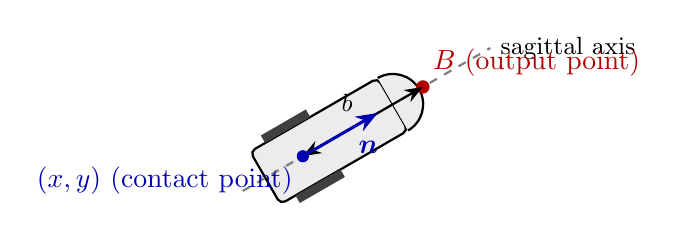
\begin{tikzpicture}[>=Stealth,thick,scale=1.1]
  \coordinate (W) at (0,0);
  \coordinate (B) at (30:1.6);
  \begin{scope}[rotate=30]
    \draw[rounded corners=2pt,fill=gray!15] (-0.5,-0.35) rectangle (1.2,0.35);
    \draw[fill=gray!15] (1.2,-0.35) arc[start angle=-90,end angle=90,radius=0.35];
    \fill[black!75] (-0.3,-0.45) rectangle (0.3,-0.35);
    \fill[black!75] (-0.3,0.35) rectangle (0.3,0.45);
    \draw[dashed,gray] (-0.8,0)--(2.5,0) node[right,black]{\small sagittal axis};
  \end{scope}
  \fill[blue!70!black] (W) circle (2pt) node[below left]{$(x,y)$ (contact point)};
  \fill[red!70!black] (B) circle (2.2pt) node[above right]{$B$ (output point)};
  \draw[<->,thick] (W)--(B) node[midway,above left]{\small $b$};
  \draw[->,blue!70!black,line width=1.1pt] (W)--($(W)+(30:1.0)$) node[pos=0.6,below right]{$\bm n$};
\end{tikzpicture}
\caption{The unicycle wheel contact point $(x,y)$ versus the off-axis point $B$ at distance $b$ along the sagittal axis: static I/O linearization drives $B$ to the goal, leaving $(x,y)$ displaced by $b$.}
\label{fig:pointB}
\end{figure}

These limitations stem directly from the nonholonomic nature of wheeled mobile robots: unlike manipulators, they do not admit \emph{universal controllers}, i.e.\ controllers able to stabilize arbitrary trajectories, whether persistent or not.
\begin{center}
\fbox{\parbox{0.88\textwidth}{\centering\bfseries Nonholonomic WMR $\implies$ No universal controller exists\\[2pt] (able to solve both tracking and regulation)}}
\end{center}
The obvious approach --- choose a path/trajectory that stops in $\bm q_d$ and then track it via feedback --- does \emph{not} work.

\begin{proposition}[Tracking a stopping trajectory fails at linear level]\label{prop:stopfail}
Let $\bm e=(e_1,e_2,e_3)$ be the tracking error expressed in the robot frame, $e_1=\cos\theta(x_d-x)+\sin\theta(y_d-y)$, $e_2=-\sin\theta(x_d-x)+\cos\theta(y_d-y)$, $e_3=\theta_d-\theta$. The linearization of the error dynamics about $\bm e=\bm 0$ is
\[
\dot{\bm e}=\begin{pmatrix}0&\omega_d&0\\-\omega_d&0&v_d\\0&0&0\end{pmatrix}\bm e+\begin{pmatrix}-1&0\\0&0\\0&-1\end{pmatrix}\begin{pmatrix}\delta v\\ \delta\omega\end{pmatrix},
\]
and when the reference comes to rest ($v_d=\omega_d=0$) it is \emph{not controllable}.
\end{proposition}

\begin{proof}
With $v_d=\omega_d=0$ the state matrix vanishes, so the controllability matrix reduces to the input matrix, whose rank is $2<3$. The lateral error $e_2$ cannot be influenced at first order.
\end{proof}

\begin{intuition}
Tracking controllers work because the reference keeps moving: while the robot rolls, a lateral error can be fixed by combining small steering and forward motion. Once the reference stops, the robot is a car with its wheels aligned: any \emph{small} correction of a sideways offset is simply not available. This is the familiar parallel-parking problem, and it is why regulation needs dedicated controllers.
\end{intuition}

\paragraph{Roadmap.}
To address regulation for the unicycle, we proceed in two successive steps:
\begin{enumerate}[leftmargin=*,nosep]
\item \textbf{Cartesian regulation}: driving the contact point $(x,y)$ to a specified Cartesian destination $(0,0)$, leaving the final orientation $\theta$ uncontrolled;
\item \textbf{Posture regulation}: driving the full configuration $(x,y,\theta)$ to a desired target $(0,0,0)$, controlling position and orientation simultaneously.
\end{enumerate}

% =====================================================================
\section{Cartesian regulation \emph{(regulation slides 3--6)}}

\subsection{Problem and geometry \emph{(regulation slide 3)}}

The first task is to drive the unicycle to a given Cartesian position (w.l.o.g.\ the origin $(0,0)$), \emph{regardless of orientation}. The relevant quantities are:
\begin{itemize}[leftmargin=*,nosep]
\item the \emph{Cartesian error} $\bm e_p=\begin{pmatrix}-x\\-y\end{pmatrix}$ (from the robot to the origin);
\item the unit vector of the sagittal axis $\bm n=\begin{pmatrix}\cos\theta\\ \sin\theta\end{pmatrix}$;
\item the projection of $\bm e_p$ on the sagittal axis, $\bm e_p^T\bm n=-x\cos\theta-y\sin\theta$;
\item the \emph{pointing error} $\gamma=\mathrm{Atan2}(y,x)+\pi-\theta$, i.e.\ the difference between the orientation of $\bm e_p$ and that of the unicycle (the angle is taken in $(-\pi,\pi]$).
\end{itemize}

\begin{figure}[ht]
\centering
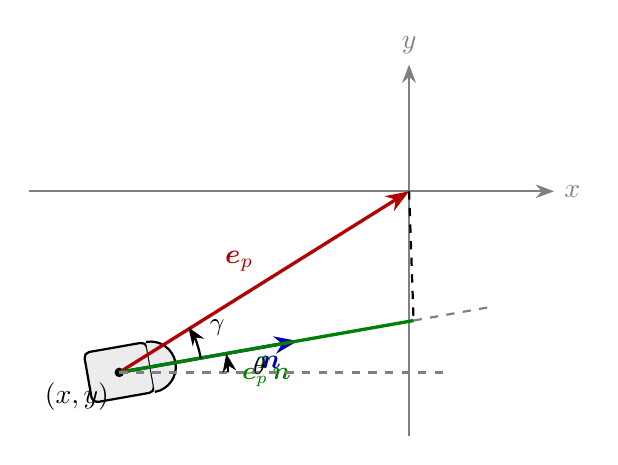
\begin{tikzpicture}[>=Stealth,thick,scale=1.15]
  \coordinate (O) at (0,0);
  \coordinate (P) at (-3.2,-2);
  \coordinate (Q) at ($(P)+(10:3.3)$);
  \draw[->,gray] (-4.2,0)--(1.6,0) node[right]{$x$};
  \draw[->,gray] (0,-2.7)--(0,1.4) node[above]{$y$};
  \begin{scope}[shift={(P)},rotate=10]
    \draw[rounded corners=2pt,fill=gray!15] (-0.35,-0.28) rectangle (0.35,0.28);
    \draw[fill=gray!15] (0.35,-0.28) arc[start angle=-90,end angle=90,radius=0.28];
  \end{scope}
  \fill (P) circle (1.5pt);
  \draw[->,red!70!black,line width=1.2pt] (P)--(O) node[midway,above left]{$\bm e_p$};
  \draw[->,blue!70!black,line width=1.2pt] (P)--($(P)+(10:2.0)$) node[pos=0.85,below]{$\bm n$};
  \draw[dashed,gray] (P)--($(P)+(10:4.2)$);
  \draw[dashed] (O)--(Q);
  \draw[very thick,green!50!black] (P)--(Q) node[midway,below,font=\small]{$\bm e_p^T\bm n$};
  \draw[dashed,gray] (P)--($(P)+(3.6,0)$);
  \draw[->] ($(P)+(1.2,0)$) arc[start angle=0,end angle=10,radius=1.2];
  \node at ($(P)+(1.55,0.07)$) {\small$\theta$};
  \draw[->] ($(P)+(0.9,0.156)$) arc[start angle=10,end angle=33.7,radius=0.9];
  \node at ($(P)+(1.08,0.5)$) {\small$\gamma$};
  \node[below left] at (P) {$(x,y)$};
\end{tikzpicture}
\caption{Geometry of Cartesian regulation: the error $\bm e_p$ points from the unicycle to the origin; its projection on the sagittal axis is $\bm e_p^T\bm n$ and the pointing error $\gamma$ is the angle between $\bm n$ and $\bm e_p$.}
\end{figure}

\subsection{Control law \emph{(regulation slide 4)}}

\begin{definition}[Cartesian regulation law]
For $k_1,k_2>0$,
\[
v=-k_1\,(x\cos\theta+y\sin\theta)=k_1\,\bm e_p^T\bm n,\qquad
\omega=k_2\,\bigl(\mathrm{Atan2}(y,x)-\theta+\pi\bigr)=k_2\,\gamma .
\]
\end{definition}

The law has a clear geometrical interpretation:
\begin{itemize}[leftmargin=*,nosep]
\item $v$ is proportional to the orthogonal \emph{projection} of the Cartesian error $\bm e_p$ on the sagittal axis;
\item $\omega$ is proportional to the \emph{pointing error}, i.e.\ the difference between the orientation of $\bm e_p$ and that of the unicycle.
\end{itemize}

\begin{intuition}
Imagine pulling a shopping cart towards a target: the further the target is \emph{straight ahead}, the faster you push; you steer in proportion to how far off to the side it is. Numbers: with $k_1=1$, $k_2=2$ and start $(x,y,\theta)=(-4,-2,0)$ we get $\bm e_p^T\bm n=4$, so $v=4$, and $\gamma=\mathrm{Atan2}(-2,-4)+\pi\approx0.46$ rad, so $\omega\approx0.93$ rad/s: the robot drives forward while turning left towards the origin. If the target is \emph{behind} the robot, $\bm e_p^T\bm n<0$ and $v$ is negative: the unicycle simply backs up.
\end{intuition}

\subsection{Brush-up: Lyapunov stability of nonlinear systems \emph{(background to regulation slide 5)}}\label{sec:lyap}

Consider an autonomous nonlinear system $\dot{\bm x}=\bm f(\bm x)$ with $\bm f$ locally Lipschitz and an equilibrium at the origin, $\bm f(\bm 0)=\bm 0$ (any other equilibrium $\bm x_e$ is brought to the origin by a translation of coordinates).

\paragraph{Why Lyapunov's indirect method (linearization) fails here.}
Before studying Lyapunov's direct method, let us address why stability cannot simply be proven via linearization:
\begin{itemize}[leftmargin=*]
\item In \emph{Lyapunov's indirect method}, one linearizes the system about an equilibrium point $\bm x_e$, obtaining $\dot{\delta\bm x} = \bm A\,\delta\bm x$ with $\bm A = \frac{\partial\bm f}{\partial\bm x}\big|_{\bm x_e}$. If all eigenvalues of $\bm A$ have strictly negative real parts ($\mathrm{Re}[\lambda_i] < 0$), the equilibrium is asymptotically stable for the nonlinear system. If at least one eigenvalue has $\mathrm{Re}[\lambda_i] > 0$, it is unstable.
\item When one or more eigenvalues lie on the imaginary axis ($\mathrm{Re}[\lambda_i] = 0$) and none in the open right-half plane, the system falls into the \textbf{critical case of Lyapunov theory}. In this critical case, linearization provides no information on stability: the outcome depends entirely on higher-order nonlinear terms.
\end{itemize}
In Cartesian regulation, every configuration $(0,0,\theta)$ is an equilibrium (the entire $\theta$-axis is an equilibrium set), so linearizing the closed-loop system about any such point yields eigenvalues with zero real parts ($\mathrm{Re}[\lambda]=0$). We are therefore squarely in the critical case, which renders the indirect method inconclusive and makes the \textbf{Lyapunov direct method} necessary.

\begin{definition}[Stability notions]
The equilibrium $\bm x=\bm 0$ is
\begin{itemize}[leftmargin=*,nosep]
\item \emph{stable} if for every $\varepsilon>0$ there is $\delta>0$ such that $\|\bm x(0)\|<\delta\Rightarrow\|\bm x(t)\|<\varepsilon$ for all $t\ge0$;
\item \emph{asymptotically stable} (AS) if it is stable and there is $\delta'>0$ such that $\|\bm x(0)\|<\delta'\Rightarrow\bm x(t)\to\bm 0$;
\item \emph{globally asymptotically stable} (GAS) if $\bm x(t)\to\bm 0$ for every initial condition;
\item \emph{exponentially stable} if $\|\bm x(t)\|\le k\|\bm x(0)\|e^{-\lambda t}$ for some $k,\lambda>0$.
\end{itemize}
\end{definition}

\begin{figure}[ht]
\centering
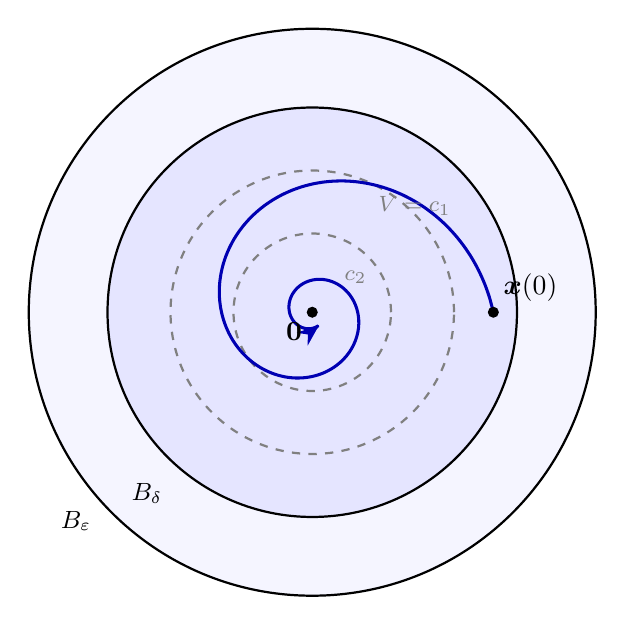
\begin{tikzpicture}[>=Stealth,thick,scale=1.0]
  \draw[fill=blue!4] (0,0) circle (3.6);
  \draw[fill=blue!10] (0,0) circle (2.6);
  \draw[dashed,gray] (0,0) circle (1.8);
  \draw[dashed,gray] (0,0) circle (1.0);
  \draw[->,blue!70!black,line width=1.1pt,smooth,samples=140,domain=0:11.5]
     plot ({2.3*exp(-0.22*\x)*cos(\x r)},{2.3*exp(-0.22*\x)*sin(\x r)});
  \fill (2.3,0) circle (2pt) node[above right]{$\bm x(0)$};
  \fill (0,0) circle (2pt) node[below left]{$\bm 0$};
  \node[font=\small] at (-2.1,-2.3) {$B_\delta$};
  \node[font=\small] at (-3.0,-2.65) {$B_\varepsilon$};
  \node[font=\footnotesize,gray] at (1.3,1.35) {$V=c_1$};
  \node[font=\footnotesize,gray] at (0.55,0.45) {$c_2$};
\end{tikzpicture}
\caption{Stability and Lyapunov level sets: a trajectory starting in $B_\delta$ never leaves $B_\varepsilon$ and, if $\dot V<0$, crosses the level sets $V=c$ (dashed, $c_1>c_2$) inwards towards the origin.}
\end{figure}

\begin{definition}[Definite and semidefinite functions]
Let $W:D\to\R$ be continuous on a neighborhood $S(\bm x_e,r)$ of $\bm x_e$, with $W(\bm x_e)=0$. We recall that:
\begin{itemize}[leftmargin=*,nosep]
\item $W$ is \emph{positive definite} (PD) in $S(\bm x_e,r)$ if $W(\bm x)>0$ for all $\bm x\in S(\bm x_e,r)\setminus\{\bm x_e\}$;
\item $W$ is \emph{positive semidefinite} (PSD) in $S(\bm x_e,r)$ if $W(\bm x)\ge0$ for all $\bm x\in S(\bm x_e,r)$ (so $W$ may vanish at states $\bm x\ne\bm x_e$);
\item $W$ is \emph{negative (semi)definite} if $-W$ is positive (semi)definite;
\item $W$ is \emph{radially unbounded} if $W(\bm x)\to\infty$ as $\|\bm x\|\to\infty$.
\end{itemize}
The derivative of a $C^1$ function along the system trajectories is $\dot V(\bm x)=\frac{\partial V}{\partial\bm x}\,\bm f(\bm x)$.
\end{definition}

\begin{theorem}[Lyapunov's direct method]\label{thm:lyap}
Let $V:D\to\R$ be $C^1$ and positive definite. Then
\begin{enumerate}[label=(\roman*),leftmargin=*,nosep]
\item $\dot V\le0$ on $D$ (NSD) $\Rightarrow$ $\bm 0$ is stable;
\item $\dot V<0$ for $\bm x\ne\bm 0$ (ND) $\Rightarrow$ $\bm 0$ is asymptotically stable;
\item $D=\R^n$, $V$ radially unbounded and $\dot V$ ND $\Rightarrow$ $\bm 0$ is globally asymptotically stable.
\end{enumerate}
\end{theorem}

\begin{proof}[Sketch of (i)]
Given $\varepsilon$, pick $r<\varepsilon$ with $B_r\subset D$ and let $m=\min_{\|\bm x\|=r}V>0$ (positive definiteness). By continuity of $V$ and $V(\bm 0)=0$ there is $\delta$ with $V<m$ on $B_\delta$. Along a trajectory starting in $B_\delta$, $V$ is nonincreasing, hence stays below $m$, so the trajectory cannot reach the sphere $\|\bm x\|=r$: it remains in $B_r\subset B_\varepsilon$.
\end{proof}

\begin{intuition}
Think of $V$ as the \emph{energy} (or the height of a bowl) and of the system as a ball with friction. If energy never increases ($\dot V\le0$), a ball started close to the bottom with little energy cannot climb far: that is stability. If energy \emph{strictly} decreases away from the bottom, friction is acting everywhere and the ball must come to rest at the bottom: asymptotic stability. The great advantage is that one never solves the differential equation: only the sign of $\dot V=\nabla V^T\bm f$ is needed.
\end{intuition}

\begin{example}\label{ex:cubic}
$\dot x=-x^3$. With $V=\frac12x^2$ (PD, radially unbounded) we get $\dot V=-x^4<0$ for $x\ne0$: the origin is GAS (though not exponentially, since the linearization is $\dot x=0$).
\end{example}

\paragraph{When $\dot V$ is only negative semidefinite: LaSalle versus Barbalat.}
Often $\dot V$ vanishes on a whole set of states, so Theorem~\ref{thm:lyap}(ii) does not apply directly. Usually, one resorts to \emph{LaSalle's invariance principle} (Theorem~\ref{thm:lasalle}). However, LaSalle's theorem strictly requires a \textbf{compact} (bounded and closed) positively invariant set $\Omega$.
In Cartesian regulation, our Lyapunov candidate is
\[
V(\bm q)=\tfrac{1}{2}(x^2+y^2)\qquad (\bm q=(x,y,\theta)^T\in\R^3).
\]
Notice that $V(\bm q)=0$ for all points $(0,0,\theta)^T$, i.e.\ along the \emph{entire vertical $\theta$-axis} (Figure~\ref{fig:vpsd}). Hence $V$ is only \textbf{positive semidefinite (PSD)} in the unicycle state space $\R^3$. Consequently, its sublevel sets $\{\bm q\in\R^3 : V(\bm q)\le c\}$ are cylinders that extend infinitely along $\theta$, violating the compactness hypothesis of LaSalle's principle! For that reason, we turn to \textbf{Barbalat's lemma}.

\begin{figure}[ht]
\centering
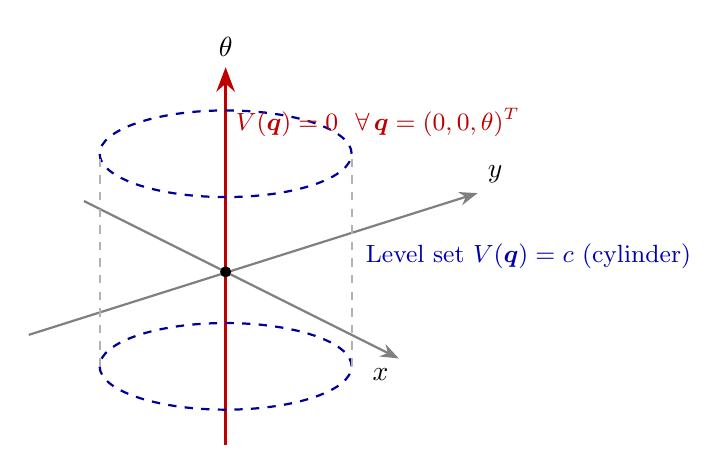
\begin{tikzpicture}[>=Stealth,thick,scale=1.0]
  \draw[->,gray] (-2.5,-0.8)--(3.2,1.0) node[above right,black]{$y$};
  \draw[->,gray] (-1.8,0.9)--(2.2,-1.1) node[below left,black]{$x$};
  \draw[->,line width=1.3pt,red!75!black] (0,-2.2)--(0,2.6) node[above,black]{$\theta$};
  \fill (0,0) circle (2pt);
  \draw[dashed,blue!60!black] (0,1.5) ellipse (1.6cm and 0.55cm);
  \draw[dashed,blue!60!black] (0,-1.2) ellipse (1.6cm and 0.55cm);
  \draw[dashed,gray!60] (-1.6,-1.2)--(-1.6,1.5);
  \draw[dashed,gray!60] (1.6,-1.2)--(1.6,1.5);
  \node[right,red!75!black,font=\small] at (0,1.9) {$V(\bm q)=0\ \ \forall\,\bm q=(0,0,\theta)^T$};
  \node[right,blue!70!black,font=\small] at (1.65,0.2) {Level set $V(\bm q)=c$ (cylinder)};
\end{tikzpicture}
\caption{The Lyapunov candidate $V(\bm q)=\frac{1}{2}(x^2+y^2)$ in configuration space $(x,y,\theta)$: $V=0$ along the entire vertical $\theta$-axis, so $V$ is only positive \emph{semidefinite} (PSD) in $\R^3$. Its sublevel sets are infinite cylinders along $\theta$, violating the compactness required by LaSalle's principle.}
\label{fig:vpsd}
\end{figure}

\begin{theorem}[LaSalle's invariance principle]\label{thm:lasalle}
Let $\Omega$ be a compact positively invariant set of $\dot{\bm x}=\bm f(\bm x)$ and $V$ a $C^1$ function with $\dot V\le0$ on $\Omega$. Let $E=\{\bm x\in\Omega:\dot V(\bm x)=0\}$ and let $M$ be the largest invariant set contained in $E$. Then every solution starting in $\Omega$ converges to $M$. In particular, if $M=\{\bm 0\}$ (and $V$ is PD) the origin is asymptotically stable.
\end{theorem}

\begin{example}\label{ex:osc}
Damped oscillator $\ddot x+\dot x+x=0$, i.e.\ $\dot x_1=x_2$, $\dot x_2=-x_1-x_2$. With $V=\frac12(x_1^2+x_2^2)$, $\dot V=-x_2^2\le0$ only NSD. On $E=\{x_2=0\}$ the dynamics give $\dot x_2=-x_1$, which keeps $x_2=0$ only if $x_1=0$: the largest invariant set in $E$ is $M=\{\bm 0\}$, so the origin is (globally) asymptotically stable.
\end{example}

\paragraph{Pedagogical motivation of Barbalat's lemma.}
To appreciate why Barbalat's lemma is needed, consider the following general result for bounded monotonic functions:
\begin{proposition}[Convergence of bounded monotonic functions]
If a function $f:\R_{\ge0}\to\R$ is always non-negative ($f(t)\ge0$) and its time derivative is always non-positive ($\dot f(t)\le0$), then $f(t)$ is non-increasing and bounded below, so $f(t)$ tends to a finite limit $\bar f\ge0$ as $t\to\infty$:
\[
f(t)\ge0,\quad \dot f(t)\le0 \implies \lim_{t\to\infty}f(t)=\bar f .
\]
\end{proposition}

Intuitively, one might jump to the conclusion that if $f(t)$ settles to a constant limit $\bar f$, its rate of change must vanish ($\dot f(t)\to0$). \textbf{However, this is not true in general}:
\[
f(t)\ge0,\quad \dot f(t)\le0 \implies f(t)\to\bar f \not\implies \dot f(t)\to0 .
\]
A function can converge while its derivative oscillates violently or produces vanishingly narrow spikes whose area under the curve is finite without $\dot f$ going to zero. For example, $f(t)=e^{-t}\sin(e^{2t})$ converges to zero, but its derivative $\dot f(t)=-e^{-t}\sin(e^{2t})+2e^t\cos(e^{2t})$ oscillates with an amplitude growing as $e^t$, which is unbounded as $t\to\infty$.
Barbalat's lemma provides the missing condition: if, in addition, the second time derivative is bounded ($|\ddot f(t)|\le b$, which implies that $\dot f(t)$ is uniformly continuous), then indeed $\dot f(t)\to0$ as $t\to\infty$.

\begin{lemma}[Barbalat]\label{lem:barbalat}
If $f:\R_{\ge0}\to\R$ is uniformly continuous and $\lim_{t\to\infty}\int_0^tf(\tau)\,d\tau$ exists and is finite, then $f(t)\to0$.
\end{lemma}

\begin{corollary}[Lyapunov-like lemma / Barbalat in time domain]\label{cor:lyaplike}
If a $C^1$ function $V(t)$ is bounded below ($V(t)\ge0$), $\dot V(t)\le0$, and $\ddot V(t)$ is bounded ($|\ddot V(t)|\le b$, so that $\dot V$ is uniformly continuous), then
\[
\lim_{t\to\infty}\dot V(t)=0 .
\]
\end{corollary}

\begin{proof}
$V(t)=V(0)+\int_0^t\dot V$ is nonincreasing and bounded below, so it has a finite limit; apply Lemma~\ref{lem:barbalat} to $f=\dot V$.
\end{proof}

\begin{remark}
Uniform continuity cannot be dropped: $f(t)=\sin(t^2)$ has a convergent integral (Fresnel) but does not tend to zero. Note also that Barbalat's lemma only says that $\dot V\to0$; it does \emph{not} say that the state converges. One must then read the information contained in $\dot V\to0$ (e.g.\ $\rho\cos\gamma\to0$ and $\gamma\to0$) and complete the argument by hand, as done below.
\end{remark}

\begin{table}[ht]
\centering
\renewcommand{\arraystretch}{1.3}
\begin{tabular}{@{}>{\raggedright\arraybackslash}p{2.6cm}>{\raggedright\arraybackslash}p{4.3cm}>{\raggedright\arraybackslash}p{3.0cm}>{\raggedright\arraybackslash}p{4.3cm}@{}}
\toprule
\textbf{Tool} & \textbf{Hypotheses} & \textbf{Needs $V$ PD?} & \textbf{Conclusion}\\
\midrule
Lyapunov direct & $V$ PD, $\dot V\le0$ (ND for AS) & yes & stability / AS / GAS\\
LaSalle & compact invariant $\Omega$, $\dot V\le0$, autonomous, continuous $\bm f$ & not necessarily & convergence to $M\subseteq\{\dot V=0\}$\\
Barbalat & $V$ bounded below, $\dot V\le0$, $\ddot V$ bounded & no & $\dot V\to0$ (state needs extra argument)\\
\bottomrule
\end{tabular}
\caption{Tools for Lyapunov-based convergence analysis.}
\end{table}

\begin{intuition}
The three tools form a ladder of weakening assumptions. Lyapunov's theorem needs a perfect ``bowl''. LaSalle accepts a bowl with flat or friction-free spots, provided the ball cannot stay on them (the largest invariant set $M$). Barbalat is the most permissive and also works when the system is not exactly autonomous or the vector field is not continuous, but it only tells you that the friction power $\dot V$ fades out, and you must deduce from it where the ball actually is.
\end{intuition}

\subsection{Convergence analysis \emph{(regulation slide 5)}}

Does the law work? Consider the Lyapunov candidate corresponding to the squared distance of the contact point $(x,y)$ to the origin $(0,0)$:
\[
V=\tfrac12(x^2+y^2)\ge0\qquad (\text{positive semidefinite in }\R^3).
\]
Computing its time derivative along the closed-loop system trajectory:
\[
\dot V = \tfrac12(2x\dot x + 2y\dot y) = x\dot x + y\dot y = x(v\cos\theta) + y(v\sin\theta) = v(x\cos\theta + y\sin\theta).
\]
Substituting the Cartesian regulation law $v = -k_1(x\cos\theta + y\sin\theta)$:
\[
\dot V = -k_1(x\cos\theta + y\sin\theta)^2 \le 0\qquad (\text{negative semidefinite}).
\]
Since $V$ represents the Cartesian error and $\dot V\le0$, the error never increases ($V(t)\le V(0)$ for all $t\ge0$); however, because $V$ is only PSD in $(x,y,\theta)$, LaSalle's theorem cannot be applied directly. We therefore apply Barbalat's lemma through Corollary~\ref{cor:lyaplike}.

\begin{proposition}[Cartesian regulation]\label{prop:cart}
Under the Cartesian regulation law (with $\gamma$ wrapped in $(-\pi,\pi]$), the Cartesian error goes to zero: $\lim_{t\to\infty}x(t)=0$ and $\lim_{t\to\infty}y(t)=0$.
\end{proposition}

\begin{proof}
The function $V\ge0$ and $\dot V\le0$, so $V(t)$ converges to a finite limit and the coordinates $x(t),y(t)$ stay bounded.
Letting $s = x\cos\theta+y\sin\theta$, we have $\dot V = -k_1s^2$, and its second derivative is
\[
\ddot V = -2k_1s\dot s,\qquad \dot s = v + \omega(-x\sin\theta+y\cos\theta).
\]
Since $x,y$, $v = -k_1s$, and $\omega = k_2\gamma$ (with $\gamma\in(-\pi,\pi]$) are all bounded, $\dot s$ and hence $\ddot V$ are bounded.
Applying Barbalat's lemma (Corollary~\ref{cor:lyaplike}), we obtain:
\[
\lim_{t\to\infty} \dot V(t) = \lim_{t\to\infty} -k_1(x\cos\theta+y\sin\theta)^2 = 0 \iff \lim_{t\to\infty}(x\cos\theta+y\sin\theta)=0 .
\]
Recalling that the projection of the Cartesian error on the sagittal axis is $\bm e_p^T\bm n = -(x\cos\theta+y\sin\theta)$, Barbalat's lemma proves that
\[
\lim_{t\to\infty}\bm e_p^T\bm n = 0 .
\]
This states that the projection of $\bm e_p$ on the sagittal axis tends to zero (the error vector and the sagittal axis become perpendicular). However, Barbalat's lemma alone does not immediately state whether $\bm e_p$ itself goes to zero.
To resolve this, we analyze the possible steady states where $\bm e_p^T\bm n = 0$ (Figure~\ref{fig:scenarios}):
\begin{itemize}[leftmargin=*]
\item \textbf{Scenario 1 ($\bm e_p\ne\bm 0$)}: The robot is broadside to the origin, so $\bm e_p\perp\bm n$. Here $v=0$, but the pointing error is $\gamma=\pm\pi/2$. Looking at the angular velocity command:
\[
\omega = k_2\gamma = \pm k_2\frac{\pi}{2} \ne 0.
\]
Because $\omega\ne0$, the wheels must turn, rotating the unicycle away from the perpendicular configuration. Therefore, Scenario~1 is \textbf{not a steady state}.
\item \textbf{Scenario 2 ($\bm e_p=\bm 0$)}: The Cartesian error is zero, meaning the wheel contact point is at the origin $(0,0)$.
\end{itemize}
We conclude that Scenario~2 is the \textbf{only feasible steady state}, and therefore $\bm e_p(t)\to\bm 0$, i.e.\ $x(t)\to0$ and $y(t)\to0$.
\end{proof}

\begin{figure}[ht]
\centering
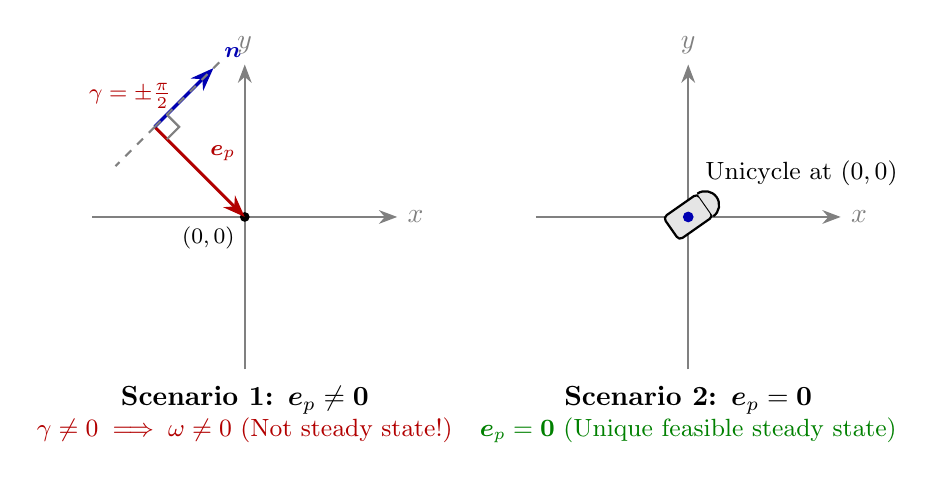
\begin{tikzpicture}[>=Stealth,thick,scale=0.88]
  \begin{scope}[shift={(-3.2,0)}]
    \draw[->,gray] (-2.2,0)--(2.2,0) node[right]{$x$};
    \draw[->,gray] (0,-2.2)--(0,2.2) node[above]{$y$};
    \fill (0,0) circle (2pt) node[below left]{\footnotesize $(0,0)$};
    \coordinate (P1) at (-1.3,1.3);
    \draw[->,red!70!black,line width=1.1pt] (P1)--(0,0) node[midway,above right]{\footnotesize $\bm e_p$};
    \draw[->,blue!70!black,line width=1.2pt] (P1)--($(P1)+(45:1.2)$) node[above right]{\footnotesize $\bm n$};
    \draw[dashed,gray] (P1)--($(P1)+(225:0.8)$);
    \draw[dashed,gray] (P1)--($(P1)+(45:1.4)$);
    \draw[gray] ($(P1)+(45:0.25)$) -- ($(P1)+(45:0.25)+(-45:0.25)$) -- ($(P1)+(-45:0.25)$);
    \node[red!70!black,font=\footnotesize] at ($(P1)+(-0.35,0.45)$) {$\gamma=\pm\frac{\pi}{2}$};
    \node[font=\bfseries,below] at (0,-2.3) {Scenario 1: $\bm e_p\ne\bm 0$};
    \node[font=\small,red!70!black,below] at (0,-2.75) {$\gamma\ne0\implies\omega\ne0$ (Not steady state!)};
  \end{scope}

  \begin{scope}[shift={(3.2,0)}]
    \draw[->,gray] (-2.2,0)--(2.2,0) node[right]{$x$};
    \draw[->,gray] (0,-2.2)--(0,2.2) node[above]{$y$};
    \begin{scope}[shift={(0,0)},rotate=35]
      \draw[rounded corners=1.5pt,fill=gray!20] (-0.3,-0.2) rectangle (0.3,0.2);
      \draw[fill=gray!20] (0.3,-0.2) arc[start angle=-90,end angle=90,radius=0.2];
    \end{scope}
    \fill[blue!70!black] (0,0) circle (2.2pt);
    \node[above right,font=\small] at (0.1,0.3) {Unicycle at $(0,0)$};
    \node[font=\bfseries,below] at (0,-2.3) {Scenario 2: $\bm e_p=\bm 0$};
    \node[font=\small,green!50!black,below] at (0,-2.75) {$\bm e_p=\bm 0$ (Unique feasible steady state)};
  \end{scope}
\end{tikzpicture}
\caption{The two possible steady-state scenarios when $\bm e_p^T\bm n\to0$: in Scenario~1 ($\bm e_p\ne\bm 0$) the sagittal axis $\bm n$ is orthogonal to $\bm e_p$, so $\gamma=\pm\pi/2$ and $\omega=k_2\gamma\ne0$, which continuously rotates the robot and breaks perpendicularity; thus Scenario~2 ($\bm e_p=\bm 0$) is the only feasible steady state.}
\label{fig:scenarios}
\end{figure}

\begin{intuition}
The distance can only decrease while $v$ is nonzero, and $v$ vanishes only when the robot is exactly broadside to the target; but there the steering term is at its maximum and immediately swings the robot back towards the target. So the robot cannot get ``stuck'' anywhere except at the goal. Note what is \emph{not} controlled: $\theta$. It ends wherever the approach direction leaves it.
\end{intuition}

\subsection{Simulation \emph{(regulation slide 6)}}

\begin{itemize}[leftmargin=*,nosep]
\item The final orientation is not controlled: it depends on the approach direction.
\item There is at most one backup maneuver (when the target starts behind the robot and $v<0$).
\end{itemize}

\begin{figure}[ht]
\centering
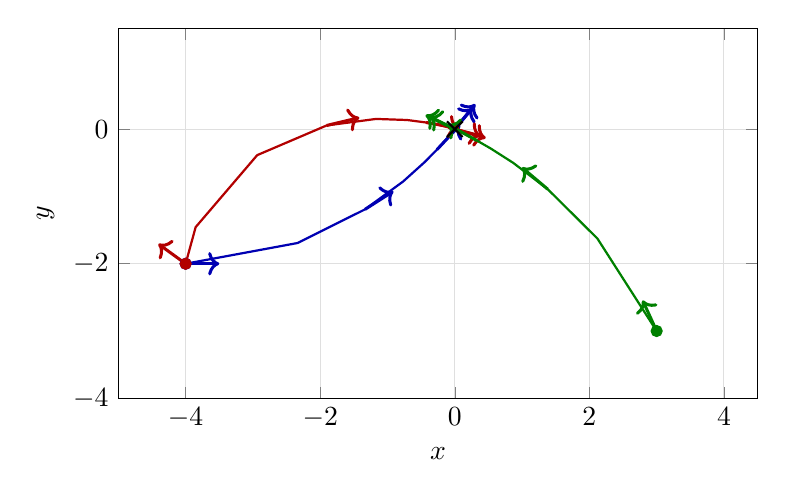
\begin{tikzpicture}
\begin{axis}[axis equal image,width=0.8\textwidth,xlabel={$x$},ylabel={$y$},grid=major,grid style={gray!25},xmin=-5,xmax=4.5,ymin=-4,ymax=1.5]
\addplot[thick,blue!70!black] coordinates {(-4.000,-2.000) (-2.337,-1.692) (-1.334,-1.192) (-0.768,-0.778) (-0.449,-0.491) (-0.265,-0.304) (-0.158,-0.187) (-0.095,-0.114) (-0.057,-0.069) (-0.035,-0.042) (-0.021,-0.026) (-0.013,-0.016)};
\draw[->,blue!70!black,line width=1.1pt] (axis cs:-4.000,-2.000)--(axis cs:-3.500,-2.000);
\draw[->,blue!70!black,line width=1.1pt] (axis cs:-1.334,-1.192)--(axis cs:-0.913,-0.923);
\draw[->,blue!70!black,line width=1.1pt] (axis cs:-0.265,-0.304)--(axis cs:0.077,0.061);
\draw[->,blue!70!black,line width=1.1pt] (axis cs:-0.057,-0.069)--(axis cs:0.264,0.314);
\draw[->,blue!70!black,line width=1.1pt] (axis cs:-0.013,-0.016)--(axis cs:0.304,0.372);
\addplot[only marks,mark=*,mark size=2pt,blue!70!black] coordinates {(-4.000,-2.000)};
\addplot[thick,red!70!black] coordinates {(-4.000,-2.000) (-3.851,-1.456) (-2.936,-0.386) (-1.904,0.055) (-1.170,0.152) (-0.708,0.136) (-0.427,0.099) (-0.258,0.066) (-0.156,0.042) (-0.094,0.026) (-0.057,0.016) (-0.035,0.010) (-0.021,0.006)};
\draw[->,red!70!black,line width=1.1pt] (axis cs:-4.000,-2.000)--(axis cs:-4.405,-1.706);
\draw[->,red!70!black,line width=1.1pt] (axis cs:-1.904,0.055)--(axis cs:-1.418,0.171);
\draw[->,red!70!black,line width=1.1pt] (axis cs:-0.427,0.099)--(axis cs:0.066,0.014);
\draw[->,red!70!black,line width=1.1pt] (axis cs:-0.094,0.026)--(axis cs:0.389,-0.102);
\draw[->,red!70!black,line width=1.1pt] (axis cs:-0.021,0.006)--(axis cs:0.460,-0.132);
\addplot[only marks,mark=*,mark size=2pt,red!70!black] coordinates {(-4.000,-2.000)};
\addplot[thick,green!50!black] coordinates {(3.000,-3.000) (2.120,-1.626) (1.380,-0.891) (0.867,-0.500) (0.535,-0.288) (0.328,-0.169) (0.200,-0.100) (0.122,-0.060) (0.074,-0.036) (0.045,-0.022) (0.027,-0.013) (0.017,-0.008)};
\draw[->,green!50!black,line width=1.1pt] (axis cs:3.000,-3.000)--(axis cs:2.792,-2.545);
\draw[->,green!50!black,line width=1.1pt] (axis cs:1.380,-0.891)--(axis cs:0.998,-0.569);
\draw[->,green!50!black,line width=1.1pt] (axis cs:0.328,-0.169)--(axis cs:-0.110,0.072);
\draw[->,green!50!black,line width=1.1pt] (axis cs:0.074,-0.036)--(axis cs:-0.374,0.186);
\draw[->,green!50!black,line width=1.1pt] (axis cs:0.017,-0.008)--(axis cs:-0.434,0.209);
\addplot[only marks,mark=*,mark size=2pt,green!50!black] coordinates {(3.000,-3.000)};
\addplot[only marks,mark=x,mark size=4pt,thick,black] coordinates {(0,0)};
\end{axis}
\end{tikzpicture}
\caption{Cartesian regulation ($k_1=1$, $k_2=2$), three initial configurations (dots); arrows show the heading along the path. The origin is reached from every start, but the final heading differs. The second run starts with the target behind the robot and backs up first.}
\label{fig:cartsim}
\end{figure}


\begin{intuition}
The three runs end at the origin with three different headings ($\approx 51^\circ$, $-16^\circ$, $154^\circ$): the controller has no mechanism to choose one. This is why a second law, which also uses the orientation error, is needed for \emph{posture} regulation.
\end{intuition}

% =====================================================================
\section{Posture regulation \emph{(regulation slides 7--10)}}

\subsection{Polar coordinates \emph{(regulation slide 7)}}

We now tackle the full posture regulation problem: driving the unicycle to a desired configuration $\bm q_d=(x_d,y_d,\theta_d)^T$, where orientation is controlled alongside position. Without loss of generality, we take the origin $\bm q_d=(0,0,0)^T$ as the goal.

In Cartesian regulation, the orientation $\theta$ was left uncontrolled because it did not enter the Lyapunov candidate $V=\frac{1}{2}(x^2+y^2)$. To design a controller that simultaneously steers position and orientation, we represent the kinematic model in \textbf{polar coordinates}. This choice decouples distance, pointing direction, and orientation error, making the control design remarkably simple.

\begin{definition}[Polar coordinates]
The polar coordinates of the unicycle with respect to the origin $\bm q_d=(0,0,0)^T$ are:
\[
\rho=\sqrt{x^2+y^2},\qquad
\gamma=\mathrm{Atan2}(y,x)-\theta+\pi,\qquad
\delta=\gamma+\theta=\mathrm{Atan2}(y,x)+\pi .
\]
Their geometric meanings are (Figure~\ref{fig:polargeom}):
\begin{itemize}[leftmargin=*,nosep]
\item $\rho$: the Euclidean \emph{distance} from the wheel contact point to the origin;
\item $\gamma$: the \emph{pointing error}, i.e.\ the angular offset between the robot heading $\theta$ and the line of sight pointing to the goal;
\item $\delta$: the \emph{orientation of the line of sight} $\bm e_p$ with respect to the world $x$ axis.
\end{itemize}
\end{definition}

The inverse transformation expressing Cartesian coordinates in terms of polar quantities is:
\[
x=-\rho\cos\delta,\qquad y=-\rho\sin\delta,\qquad \theta=\delta-\gamma .
\]

\paragraph{Note on indefiniteness at the origin.}
Because $\gamma$ and $\delta$ are computed using $\mathrm{Atan2}(y,x)$, they are \textbf{undefined at the Cartesian origin} $(x,y)=(0,0)$. However, if the polar quantities converge to zero ($\rho\to0$, $\gamma\to0$, $\delta\to0$), then the Cartesian posture also converges to the origin: $x\to0$, $y\to0$, and $\theta=\delta-\gamma\to0$.

\begin{figure}[ht]
\centering
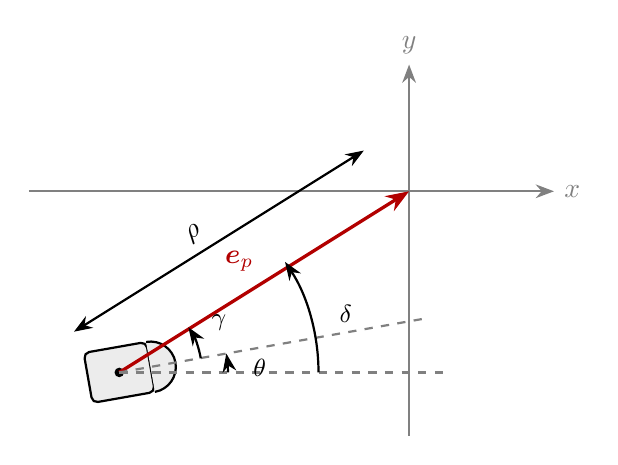
\begin{tikzpicture}[>=Stealth,thick,scale=1.15]
  \coordinate (O) at (0,0);
  \coordinate (P) at (-3.2,-2);
  \draw[->,gray] (-4.2,0)--(1.6,0) node[right]{$x$};
  \draw[->,gray] (0,-2.7)--(0,1.4) node[above]{$y$};
  \begin{scope}[shift={(P)},rotate=10]
    \draw[rounded corners=2pt,fill=gray!15] (-0.35,-0.28) rectangle (0.35,0.28);
    \draw[fill=gray!15] (0.35,-0.28) arc[start angle=-90,end angle=90,radius=0.28];
  \end{scope}
  \fill (P) circle (1.5pt);
  \draw[->,red!70!black,line width=1.2pt] (P)--(O) node[midway,above left]{$\bm e_p$};
  \draw[<->] ($(P)+(-0.5,0.45)$) -- ($(O)+(-0.5,0.45)$) node[midway,above left,sloped]{$\rho$};
  \draw[dashed,gray] (P)--($(P)+(10:3.4)$);
  \draw[dashed,gray] (P)--($(P)+(3.6,0)$);
  \draw[->] ($(P)+(1.2,0)$) arc[start angle=0,end angle=10,radius=1.2];
  \node at ($(P)+(1.55,0.05)$) {\small$\theta$};
  \draw[->] ($(P)+(0.9,0.156)$) arc[start angle=10,end angle=33.7,radius=0.9];
  \node at ($(P)+(1.1,0.55)$) {\small$\gamma$};
  \draw[->] ($(P)+(2.2,0)$) arc[start angle=0,end angle=33.7,radius=2.2];
  \node at ($(P)+(2.5,0.65)$) {\small$\delta$};
\end{tikzpicture}
\caption{Polar coordinates of the unicycle with respect to the origin: $\rho$ is the distance, $\gamma$ the pointing error and $\delta=\gamma+\theta$ the orientation of $\bm e_p$ with respect to the $x$ axis.}
\label{fig:polargeom}
\end{figure}

\begin{intuition}
Instead of asking ``where am I in the plane'', ask three questions: how far is the goal ($\rho$), how far off is my nose from pointing at it ($\gamma$), and from which side of the goal am I looking at it ($\delta$). The third angle is what encodes the final orientation: at the goal, $\theta=\delta-\gamma$, so making \emph{both} angles vanish forces $\theta=0$. The price is that the coordinates are singular at the origin itself.
\end{intuition}

\subsection{Kinematic model in polar coordinates \emph{(regulation slide 8)}}

\begin{proposition}[Kinematic model in polar coordinates]\label{prop:polarmodel}
For $\rho\neq0$, the unicycle kinematics in polar coordinates $(\rho,\gamma,\delta)$ are
\[
\dot\rho=-v\cos\gamma,\qquad
\dot\gamma=\frac{\sin\gamma}{\rho}\,v-\omega,\qquad
\dot\delta=\frac{\sin\gamma}{\rho}\,v .
\]
\end{proposition}

\begin{proof}
Let us derive each equation step by step.

\paragraph{Derivation of $\dot\rho$:}
Differentiating $\rho = (x^2+y^2)^{1/2}$ with respect to time:
\[
\dot\rho = \frac{d}{dt}(x^2+y^2)^{1/2} = \frac{1}{2}(x^2+y^2)^{-1/2}(2x\dot x + 2y\dot y) = \frac{x\dot x + y\dot y}{\sqrt{x^2+y^2}} = \frac{x\cos\theta\,v + y\sin\theta\,v}{\rho}.
\]
To simplify this expression, introduce the polar angle $\beta = \mathrm{Atan2}(y,x)$ of the position vector (Figure~\ref{fig:polarbeta}), so that
\[
x = \rho\cos\beta,\qquad y = \rho\sin\beta .
\]
Substituting into $\dot\rho$:
\[
\dot\rho = \frac{\rho\cos\beta\cos\theta\,v + \rho\sin\beta\sin\theta\,v}{\rho} = v(\cos\beta\cos\theta + \sin\beta\sin\theta) = v\cos(\beta-\theta).
\]
Recalling that $\cos\alpha = -\cos(\alpha+\pi)$ and that $\gamma = \mathrm{Atan2}(y,x)-\theta+\pi = \beta-\theta+\pi$:
\[
\cos(\beta-\theta) = -\cos(\beta-\theta+\pi) = -\cos\gamma \implies \dot\rho = -v\cos\gamma .
\]

\paragraph{Derivation of $\dot\gamma$:}
From $\gamma = \mathrm{Atan2}(y,x)-\theta+\pi$, we have
\[
\dot\gamma = \frac{d}{dt}\mathrm{Atan2}(y,x) - \dot\theta = \frac{d}{dt}\mathrm{Atan2}(y,x) - \omega .
\]
Applying the chain rule to differentiate $\mathrm{Atan2}(y,x)$:
\[
\frac{d}{dt}\mathrm{Atan2}(y,x) = \frac{\partial\mathrm{Atan2}(y,x)}{\partial x}\dot x + \frac{\partial\mathrm{Atan2}(y,x)}{\partial y}\dot y .
\]
Since $\frac{\partial\arctan(y/x)}{\partial x} = -\frac{y}{x^2+y^2}$ and $\frac{\partial\arctan(y/x)}{\partial y} = \frac{x}{x^2+y^2}$, we obtain
\[
\frac{d}{dt}\mathrm{Atan2}(y,x) = -\frac{y}{\rho^2}\dot x + \frac{x}{\rho^2}\dot y = \frac{x\dot y - y\dot x}{\rho^2} = \frac{x\sin\theta\,v - y\cos\theta\,v}{\rho^2}.
\]
Substituting $x = \rho\cos\beta$ and $y = \rho\sin\beta$:
\[
\frac{d}{dt}\mathrm{Atan2}(y,x) = \frac{v}{\rho}(\cos\beta\sin\theta - \sin\beta\cos\theta) = -\frac{v}{\rho}(\sin\beta\cos\theta - \cos\beta\sin\theta) = -\frac{v}{\rho}\sin(\beta-\theta).
\]
Using $-\sin\alpha = \sin(\alpha+\pi)$ and $\beta-\theta+\pi = \gamma$:
\[
-\sin(\beta-\theta) = \sin(\beta-\theta+\pi) = \sin\gamma \implies \frac{d}{dt}\mathrm{Atan2}(y,x) = \frac{v\sin\gamma}{\rho}.
\]
Therefore,
\[
\dot\gamma = \frac{\sin\gamma}{\rho}\,v - \omega .
\]

\paragraph{Derivation of $\dot\delta$:}
Since $\delta = \gamma+\theta$,
\[
\dot\delta = \frac{d}{dt}(\gamma+\theta) = \dot\gamma + \dot\theta = \left(\frac{\sin\gamma}{\rho}\,v - \omega\right) + \omega = \frac{\sin\gamma}{\rho}\,v .
\]
This completes the derivation of the kinematic model.
\end{proof}

\begin{figure}[ht]
\centering
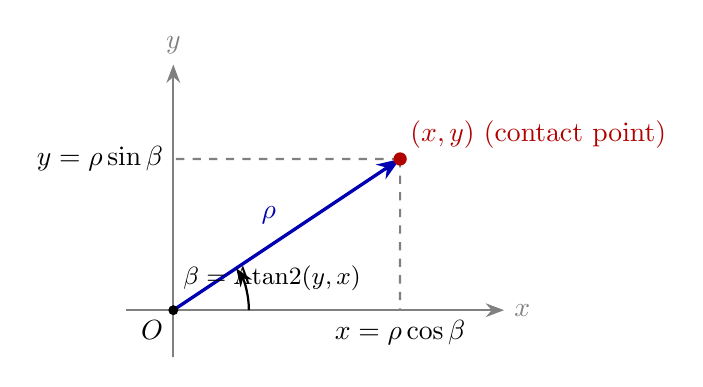
\begin{tikzpicture}[>=Stealth,thick,scale=1.2]
  \draw[->,gray] (-0.5,0)--(3.5,0) node[right]{$x$};
  \draw[->,gray] (0,-0.5)--(0,2.6) node[above]{$y$};
  \coordinate (O) at (0,0);
  \coordinate (P) at (2.4,1.6);
  \draw[dashed,gray] (P)--(2.4,0) node[below,black]{$x=\rho\cos\beta$};
  \draw[dashed,gray] (P)--(0,1.6) node[left,black]{$y=\rho\sin\beta$};
  \draw[->,line width=1.2pt,blue!70!black] (O)--(P) node[midway,above left]{$\rho$};
  \fill[red!70!black] (P) circle (2pt) node[above right]{$(x,y)$ (contact point)};
  \fill (O) circle (1.5pt) node[below left]{$O$};
  \draw[->] (0.8,0) arc[start angle=0,end angle=33.7,radius=0.8];
  \node at (18:1.1) {\small$\beta=\mathrm{Atan2}(y,x)$};
\end{tikzpicture}
\caption{Auxiliary polar angle $\beta=\mathrm{Atan2}(y,x)$: the contact point coordinates are $x=\rho\cos\beta$ and $y=\rho\sin\beta$, which simplifies the differentiation of $\rho$ and $\gamma$.}
\label{fig:polarbeta}
\end{figure}

\begin{remark}[Behavior when reaching the origin: singularity resolution]
Our ultimate control goal is to reach $(x,y,\theta)=(0,0,0)$, which corresponds to $(\rho,\gamma,\delta)\to(0,0,0)$.
Looking at the polar kinematic model, $\rho$ appears in the denominator of $\dot\gamma$ and $\dot\delta$, which might suggest a risk of divergence ($\dot\gamma\to\infty$, $\dot\delta\to\infty$) as $\rho\to0$.
However, this is \textbf{not an issue}: in the control law synthesized below, the driving velocity $v$ is chosen proportional to $\rho$ ($v = k_1\rho\cos\gamma$), so that the ratio
\[
\frac{v}{\rho} = k_1\cos\gamma
\]
remains completely bounded by $k_1$. Therefore, the coupling term
\[
\frac{\sin\gamma}{\rho}\,v = k_1\sin\gamma\cos\gamma
\]
is smooth, well-defined, and vanishes as $\gamma\to0$. The apparent kinematic singularity is effectively tamed by the control law.
\end{remark}

\subsection{Control law design via Lyapunov's direct method \emph{(regulation slides 8--9)}}

The Lyapunov direct method can be used not only as an a-posteriori verification tool, but as a \textbf{constructive synthesis method} to design the feedback control law.

\paragraph{Design procedure.}
We start by defining a candidate Lyapunov function representing the total error ``energy'':
\[
V = \tfrac{1}{2}\left(\rho^2 + \gamma^2 + \delta^2\right) > 0\qquad (\text{positive definite in polar coordinates}).
\]
Computing its time derivative along the trajectories of the polar kinematic model:
\[
\dot V = \rho\dot\rho + \gamma\dot\gamma + \delta\dot\delta .
\]
Plugging in the equations for $\dot\rho$, $\dot\gamma$, and $\dot\delta$ from Proposition~\ref{prop:polarmodel}:
\[
\dot V = \rho(-v\cos\gamma) + \gamma\left(\frac{\sin\gamma}{\rho}\,v - \omega\right) + \delta\left(\frac{\sin\gamma}{\rho}\,v\right)
= -\rho v\cos\gamma + \frac{\sin\gamma}{\rho}(\gamma+\delta)v - \gamma\omega .
\]
We now synthesize the inputs $v$ and $\omega$ in three consecutive steps:
\begin{enumerate}[leftmargin=*]
\item \textbf{Step 1: Choice of $v$.}
Examine the first term $-\rho v\cos\gamma$. To ensure this term is non-positive, we set
\[
v = k_1\rho\cos\gamma\qquad (k_1>0).
\]
This makes $-\rho v\cos\gamma = -k_1\rho^2\cos^2\gamma \le 0$. The parameter $k_1>0$ provides tuning freedom to adjust the linear approach speed. This would still work without $\rho$ in the expression, but then the robot would slow down as it approaches the origin, which is undesirable for posture regulation, and so $\rho$ will act as a gain.

\item \textbf{Step 2: Decomposition of $\omega$.}
With $v$ determined by the first term, $\dot V$ becomes:
\[
\dot V = \underbrace{-k_1\rho^2\cos^2\gamma}_{\le 0} + \underbrace{\frac{\sin\gamma}{\rho}(\gamma+\delta)v}_{\text{cross coupling}} - \underbrace{\gamma\omega}_{\text{control input}} .
\]
Because $v$ was chosen strictly to stabilize $\rho$, we cannot use it to govern the sign of the cross-coupling second term. We must therefore use the steering input $\omega$.
We decompose $\omega$ into two parts:
\[
\omega = k_2\gamma + \alpha\qquad (k_2>0),
\]
so that the control term expands to $-\gamma\omega = -k_2\gamma^2 - \gamma\alpha$, where $-k_2\gamma^2 \le 0$ acts as a stabilizing negative damping on $\gamma$.

\item \textbf{Step 3: Cross-term cancellation via $\alpha$.}
We choose the auxiliary term $\alpha$ to identically cancel the cross-coupling term:
\[
\frac{\sin\gamma}{\rho}(\gamma+\delta)v - \gamma\alpha = 0 \iff \alpha = \frac{\sin\gamma}{\gamma\rho}(\gamma+\delta)v .
\]
Substituting $v = k_1\rho\cos\gamma$:
\[
\alpha = \frac{\sin\gamma}{\gamma\rho}(\gamma+\delta)\bigl(k_1\rho\cos\gamma\bigr) = k_1\frac{\sin\gamma\cos\gamma}{\gamma}(\gamma+\delta).
\]
\end{enumerate}

Combining the terms yields the complete posture regulation law:
\begin{definition}[Posture regulation law]
For $k_1,k_2>0$,
\[
v=k_1\,\rho\cos\gamma,\qquad
\omega=k_2\,\gamma+k_1\,\frac{\sin\gamma\cos\gamma}{\gamma}\,(\gamma+\delta),
\]
where $\frac{\sin\gamma\cos\gamma}{\gamma}\to1$ as $\gamma\to0$. Compared with Cartesian regulation, $v$ has the same form (since $\rho\cos\gamma = -(x\cos\theta+y\sin\theta)$), while $\omega$ incorporates an additional correction proportional to $\gamma+\delta$.
Under this control law, the cross terms in $\dot V$ cancel identically, leaving:
\[
\dot V = -k_1\rho^2\cos^2\gamma - k_2\gamma^2 \le 0\qquad (\text{negative semidefinite}).
\]
\end{definition}

\begin{algorithm}[Posture regulation]
At each control instant:
\begin{enumerate}[leftmargin=*,nosep]
\item measure $(x,y,\theta)$ and compute $\rho=\sqrt{x^2+y^2}$, $\gamma=\mathrm{Atan2}(y,x)-\theta+\pi$ (wrapped in $(-\pi,\pi]$) and $\delta=\gamma+\theta$;
\item compute $v=k_1\rho\cos\gamma$ and $\omega=k_2\gamma+k_1\frac{\sin\gamma\cos\gamma}{\gamma}(\gamma+\delta)$, using the limit value $1$ for the fraction when $\gamma=0$;
\item send $(v,\omega)$ to the unicycle.
\end{enumerate}
\end{algorithm}

\begin{intuition}
The new term in $\omega$ is what takes care of the final orientation. Numerical example at $(x,y,\theta)=(-4,-2,0)$ with $k_1=1$, $k_2=3$: $\rho\approx4.47$, $\gamma=\delta\approx0.46$, so $v\approx4.0$ and $\omega\approx1.39+0.80=2.19$ rad/s, against $1.39$ rad/s for the pure pointing term. The robot turns \emph{more} than needed to point at the origin, so that it arrives rotated in the correct direction, in the style of a car aligning with a parking spot as it approaches.
\end{intuition}

\subsection{Convergence analysis and Brockett's theorem \emph{(regulation slide 9)}}

\begin{proposition}[Posture regulation]\label{prop:post}
Under the posture regulation law, $\dot V=-k_1\cos^2\!\gamma\,\rho^2-k_2\gamma^2\le0$ (negative semidefinite), and $\rho,\gamma,\delta\to0$; hence $x,y,\theta\to0$.
\end{proposition}

\begin{proof}
Substituting the control law, the closed-loop system is
\[
\dot\rho=-k_1\rho\cos^2\!\gamma,\qquad
\dot\gamma=-k_2\gamma-k_1\frac{\sin\gamma\cos\gamma}{\gamma}\,\delta,\qquad
\dot\delta=k_1\sin\gamma\cos\gamma .
\]
Then
\[
\dot V=\rho\dot\rho+\gamma\dot\gamma+\delta\dot\delta=-k_1\rho^2\cos^2\!\gamma-k_2\gamma^2-k_1\sin\gamma\cos\gamma\,\delta+k_1\delta\sin\gamma\cos\gamma=-k_1\cos^2\!\gamma\,\rho^2-k_2\gamma^2 .
\]
$V$ is positive definite and $\dot V$ only negative semidefinite, so by Barbalat's lemma $\dot V\to0$, i.e.\ $\rho\cos\gamma\to0$ and $\gamma\to0$; thus also $\rho\to0$. For $\delta$: $\gamma\to0$ and (again by Barbalat, since $\ddot\gamma$ is bounded) $\dot\gamma\to0$, so from the expression of $\dot\gamma$ the term $k_1\frac{\sin\gamma\cos\gamma}{\gamma}\delta\to0$; as the fraction tends to $1$, $\delta\to0$.
\end{proof}

\begin{remark}[Discontinuity of the control law in Cartesian coordinates]
The control law was designed in polar coordinates $(\rho,\gamma,\delta)$. Once mapped back to the original Cartesian state $\bm q=(x,y,\theta)^T$, the law is \textbf{discontinuous} at the origin $(0,0,0)$ because $\mathrm{Atan2}(y,x)$ has an essential singularity at $x=y=0$.
\end{remark}

\begin{remark}[Practical behavior: why discontinuity is not an issue]
In real-world implementations, \textbf{this discontinuity is never practically encountered}:
\begin{itemize}[leftmargin=*,nosep]
\item The physical robot asymptotically converges toward the origin, but because of discrete-time sampling, sensor resolution limits, and physical disturbances, the state never lands mathematically on the exact singular point $(x,y)=(0,0)$.
\item A microscopic residual error always persists, keeping $\rho>0$ and the control inputs well-defined at all times until the control task is terminated.
\end{itemize}
\end{remark}

This discontinuity is by no means an accident of the chosen polar coordinates; it is a fundamental consequence of nonholonomy:

\begin{theorem}[Brockett]\label{thm:brockett}
Consider a driftless system $\dot{\bm q}=\bm G(\bm q)\bm u$ with $\mathrm{rank}\,\bm G=m<n$. A necessary condition for the existence of a continuous time-invariant feedback $\bm u=\bm k(\bm q)$ asymptotically stabilizing an equilibrium $\bm q_d$ is that the map $(\bm q,\bm u)\mapsto\bm G(\bm q)\bm u$ be onto an open neighborhood of $\bm 0$. This fails for nonholonomic systems; hence all posture stabilizers must be \emph{discontinuous with respect to the state} or \emph{time-varying}.
\end{theorem}

\begin{proof}[Verification for the unicycle]
Around $\theta=0$ we have $\cos\theta\neq0$. The velocity vector
\[
(\dot x,\dot y,\dot\theta)^T = (v\cos\theta,\, v\sin\theta,\, \omega)^T
\]
can match $(0,\varepsilon,0)^T$ only if $v\cos\theta=0$, which implies $v=0$, and therefore $\dot y=0\ne\varepsilon$. Consequently, points of the form $(0,\varepsilon,0)^T$, however small $\varepsilon>0$ is chosen, are never in the image of the velocity map.
\end{proof}

\begin{intuition}
A continuous static feedback would give small controls near the goal and thus small velocities, but a small \emph{sideways} offset can only be fixed by moving \emph{away} and coming back with a different heading (the parallel-parking manoeuvre), which is a large motion, not a small one. Two ways out: allow the feedback to jump (discontinuous, as here: the law is not defined at $\rho=0$) or let it depend on time (time-varying laws oscillate to generate the sideways motion).
\end{intuition}

\subsection{Simulation \emph{(regulation slide 10)}}

\begin{itemize}[leftmargin=*,nosep]
\item The final orientation is zeroed as well, regardless of the initial configuration.
\item There is at most one backup maneuver.
\end{itemize}

\begin{figure}[ht]
\centering
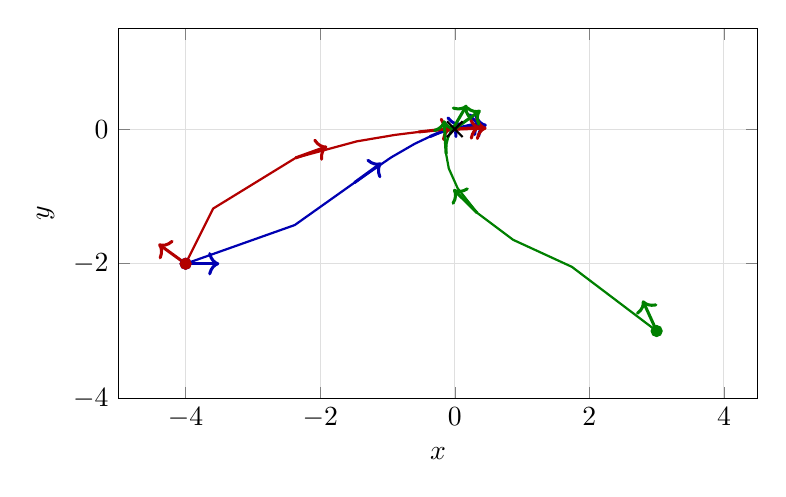
\begin{tikzpicture}
\begin{axis}[axis equal image,width=0.8\textwidth,xlabel={$x$},ylabel={$y$},grid=major,grid style={gray!25},xmin=-5,xmax=4.5,ymin=-4,ymax=1.5]
\addplot[thick,blue!70!black] coordinates {(-4.000,-2.000) (-2.378,-1.425) (-1.491,-0.795) (-0.946,-0.420) (-0.595,-0.217) (-0.371,-0.111) (-0.229,-0.056) (-0.141,-0.028) (-0.086,-0.014) (-0.052,-0.007) (-0.032,-0.004) (-0.019,-0.002)};
\draw[->,blue!70!black,line width=1.1pt] (axis cs:-4.000,-2.000)--(axis cs:-3.500,-2.000);
\draw[->,blue!70!black,line width=1.1pt] (axis cs:-1.491,-0.795)--(axis cs:-1.087,-0.501);
\draw[->,blue!70!black,line width=1.1pt] (axis cs:-0.371,-0.111)--(axis cs:0.090,0.084);
\draw[->,blue!70!black,line width=1.1pt] (axis cs:-0.086,-0.014)--(axis cs:0.401,0.099);
\draw[->,blue!70!black,line width=1.1pt] (axis cs:-0.019,-0.002)--(axis cs:0.476,0.062);
\addplot[only marks,mark=*,mark size=2pt,blue!70!black] coordinates {(-4.000,-2.000)};
\addplot[thick,red!70!black] coordinates {(-4.000,-2.000) (-3.591,-1.180) (-2.365,-0.427) (-1.455,-0.181) (-0.886,-0.085) (-0.539,-0.042) (-0.327,-0.021) (-0.198,-0.010) (-0.120,-0.005) (-0.073,-0.003) (-0.044,-0.001) (-0.027,-0.001)};
\draw[->,red!70!black,line width=1.1pt] (axis cs:-4.000,-2.000)--(axis cs:-4.405,-1.706);
\draw[->,red!70!black,line width=1.1pt] (axis cs:-2.365,-0.427)--(axis cs:-1.895,-0.258);
\draw[->,red!70!black,line width=1.1pt] (axis cs:-0.539,-0.042)--(axis cs:-0.042,0.013);
\draw[->,red!70!black,line width=1.1pt] (axis cs:-0.120,-0.005)--(axis cs:0.379,0.025);
\draw[->,red!70!black,line width=1.1pt] (axis cs:-0.027,-0.001)--(axis cs:0.473,0.016);
\addplot[only marks,mark=*,mark size=2pt,red!70!black] coordinates {(-4.000,-2.000)};
\addplot[thick,green!50!black] coordinates {(3.000,-3.000) (1.740,-2.046) (0.866,-1.644) (0.334,-1.245) (0.043,-0.879) (-0.089,-0.584) (-0.129,-0.367) (-0.123,-0.221) (-0.100,-0.127) (-0.073,-0.071) (-0.051,-0.039) (-0.034,-0.020) (-0.022,-0.011)};
\draw[->,green!50!black,line width=1.1pt] (axis cs:3.000,-3.000)--(axis cs:2.792,-2.545);
\draw[->,green!50!black,line width=1.1pt] (axis cs:0.334,-1.245)--(axis cs:-0.021,-0.894);
\draw[->,green!50!black,line width=1.1pt] (axis cs:-0.129,-0.367)--(axis cs:-0.159,0.132);
\draw[->,green!50!black,line width=1.1pt] (axis cs:-0.073,-0.071)--(axis cs:0.180,0.360);
\draw[->,green!50!black,line width=1.1pt] (axis cs:-0.022,-0.011)--(axis cs:0.384,0.281);
\addplot[only marks,mark=*,mark size=2pt,green!50!black] coordinates {(3.000,-3.000)};
\addplot[only marks,mark=x,mark size=4pt,thick,black] coordinates {(0,0)};
\end{axis}
\end{tikzpicture}
\caption{Posture regulation ($k_1=1$, $k_2=3$) from the same three initial configurations (dots): the robot reaches the origin \emph{and} the final heading is $\theta=0$ in all cases (arrows along the $x$ axis at the origin).}
\label{fig:postsim}
\end{figure}



% =====================================================================
\part{Mobile manipulators}

\section{Mobile manipulators \emph{(manipulator slides 1--2)}}

\begin{definition}[Mobile manipulator]
A \emph{mobile manipulator} (MM) is a robot made of a mobile base carrying one or more manipulators. In the vast majority of cases the base is \emph{wheeled} and the manipulator is an \emph{articulated arm}. Its configuration is
\[
\bm q=(\qbase,\qarm),
\]
where $\qbase\in\R^{n_b}$ collects the $n_b$ generalized coordinates of the base (e.g.\ $(x,y,\theta)$ for a planar vehicle) and $\qarm\in\R^{n_m}$ collects the $n_m$ joint coordinates of the arm. The total number of coordinates is $n=n_b+n_m$.
\end{definition}

\begin{figure}[ht]
\centering
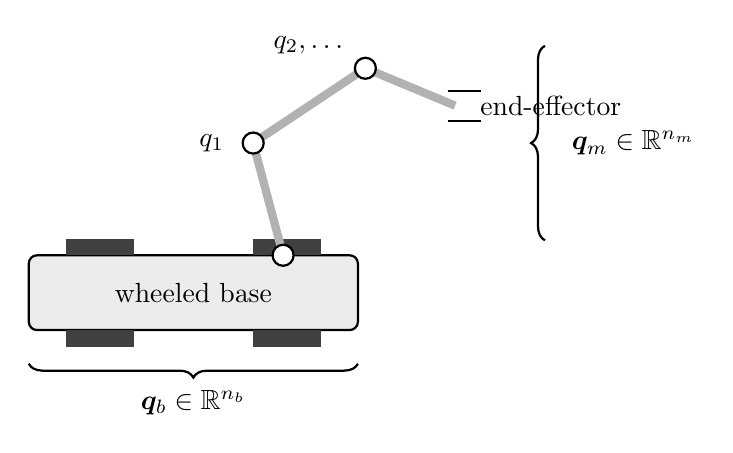
\begin{tikzpicture}[>=Stealth,thick,scale=0.95]
  % base
  \draw[rounded corners=3pt,fill=gray!15] (0,0) rectangle (4.4,1);
  \fill[black!75] (0.5,-0.22) rectangle (1.4,0);
  \fill[black!75] (3.0,-0.22) rectangle (3.9,0);
  \fill[black!75] (0.5,1) rectangle (1.4,1.22);
  \fill[black!75] (3.0,1) rectangle (3.9,1.22);
  \node at (2.2,0.5) {wheeled base};
  % arm
  \coordinate (A0) at (3.4,1);
  \coordinate (A1) at (3.0,2.5);
  \coordinate (A2) at (4.5,3.5);
  \coordinate (A3) at (5.7,3.0);
  \draw[line width=3pt,gray!60] (A0)--(A1)--(A2)--(A3);
  \foreach \p in {A0,A1,A2}{\draw[fill=white] (\p) circle (4pt);}
  \draw (A3)++(-0.1,0.2)--++(0.45,0.0)  (A3)++(-0.1,-0.2)--++(0.45,0.0);
  \node[right] at (5.9,3.0) {end-effector};
  \node[left] at (2.75,2.5) {$q_1$};
  \node[above left] at (4.4,3.55) {$q_2,\dots$};
  % labels
  \draw[decorate,decoration={brace,mirror,amplitude=5pt}] (0,-0.45)--(4.4,-0.45)
        node[midway,below=6pt]{$\qbase\in\R^{n_b}$};
  \draw[decorate,decoration={brace,amplitude=5pt}] (6.9,1.2)--(6.9,3.8)
        node[midway,right=6pt]{$\qarm\in\R^{n_m}$};
\end{tikzpicture}
\caption{Structure of a mobile manipulator: the configuration splits into base coordinates $\qbase$ and arm joint coordinates $\qarm$.}
\end{figure}

\begin{intuition}
Think of an MM as a ``manipulator that can move its own shoulder''. The base extends the workspace of the arm enormously (the arm can reach anything the base can drive to), and, as we will see, it also adds degrees of freedom that remove the singularities of the arm alone. The price is that the base is usually \emph{nonholonomic}: it has fewer controls than coordinates, so the two halves of the robot behave very differently.
\end{intuition}

% =====================================================================
\section{Kinematic model \emph{(manipulator slide 3)}}

A mobile manipulator is the mechanical composition of two fundamentally different kinematic subsystems:
\begin{enumerate}[leftmargin=*,nosep]
\item a \textbf{constrained robot} (the mobile base), subject to nonholonomic velocity constraints;
\item an \textbf{unconstrained robot} (the manipulator arm), whose joints are directly actuated without differential constraints.
\end{enumerate}

\subsection*{Constrained robot: the mobile base}

A kinematic system is called \emph{constrained} when its generalized velocities cannot be commanded arbitrarily in all directions, but must satisfy non-integrable (nonholonomic) constraints.

\begin{example}[Constrained robot: unicycle base]
Consider a unicycle (or differential-drive vehicle) moving on a plane. Its configuration is described by the base generalized coordinates
\[
\qbase = (x, y, \theta)^T \in \R^{n_b},\qquad (n_b = 3),
\]
where $(x,y)$ represents the position of the wheel contact point and $\theta$ is the vehicle heading.
The wheels cannot slide sideways (pure rolling and no slip condition), imposing the nonholonomic constraint in Pfaffian form:
\[
\bm A_b(\qbase)\,\dot{\qbase} = \dot x\sin\theta - \dot y\cos\theta = \begin{pmatrix}\sin\theta & -\cos\theta & 0\end{pmatrix}\begin{pmatrix}\dot x\\ \dot y\\ \dot\theta\end{pmatrix} = 0.
\]
The subspace of admissible generalized velocities at configuration $\qbase$ is the null space of $\bm A_b(\qbase)$, which has dimension $m_b = n_b - 1 = 2$.
Choosing a basis for $\ker\bm A_b(\qbase)$, the admissible velocities are parameterized by $m_b = 2$ \emph{pseudovelocities} $\ubase = (v, \omega)^T$, where $v$ is the driving linear velocity and $\omega$ is the steering angular velocity:
\[
\dot{\qbase} = \begin{pmatrix}\dot x\\ \dot y\\ \dot\theta\end{pmatrix} = \begin{pmatrix}\cos\theta & 0\\ \sin\theta & 0\\ 0 & 1\end{pmatrix}\begin{pmatrix}v\\ \omega\end{pmatrix} = \Gbase(\qbase)\,\ubase .
\]
Because $m_b = 2 < 3 = n_b$, the base is kinematically \textbf{constrained}: instantaneous motion in the lateral direction $\begin{pmatrix}-\sin\theta & \cos\theta & 0\end{pmatrix}^T$ is strictly forbidden, even though the vehicle can reach any configuration $(x,y,\theta)$ through appropriate maneuvers.
\end{example}

\subsection*{Unconstrained robot: the manipulator arm}

In contrast, a standard articulated manipulator mounted on the base has joints that are independently driven by individual actuators.

\begin{example}[Unconstrained robot: articulated manipulator arm]
Consider a serial manipulator with $n_m$ revolute (or prismatic) joints, with joint coordinates
\[
\qarm = (q_1, q_2, \dots, q_{n_m})^T \in \R^{n_m}.
\]
Unlike the wheeled base, the arm is subject to \textbf{no nonholonomic constraints}. Each joint velocity $\dot q_j$ can be independently and directly commanded by the joint velocity inputs:
\[
\uarm = (\dot q_1, \dot q_2, \dots, \dot q_{n_m})^T \in \R^{m_m},\qquad (m_m = n_m).
\]
Consequently, the kinematic model of the arm is simply:
\[
\dot{\qarm} = \bm I_{n_m}\,\uarm = \uarm .
\]
Because the number of velocity inputs equals the dimension of the configuration space ($m_m = n_m$), the robot is kinematically \textbf{unconstrained}: at any configuration $\qarm$, the arm can instantaneously move with any generalized velocity $\dot{\qarm}\in\R^{n_m}$ without restriction. For example, for a planar 2R arm ($n_m = 2$), $\qarm = (q_1, q_2)^T$ and $\dot{\qarm} = \begin{pmatrix}1 & 0\\ 0 & 1\end{pmatrix}\begin{pmatrix}\dot q_1\\ \dot q_2\end{pmatrix}$.
\end{example}

\subsection*{Combined kinematic model}

\begin{definition}[Kinematic model of a mobile manipulator]
Stacking the constrained base subsystem and the unconstrained arm subsystem, the complete mobile manipulator configuration is $\bm q = (\qbase, \qarm) \in \R^{n}$ with $n = n_b + n_m$, driven by the stacked velocity inputs $\bm u = (\ubase, \uarm) \in \R^{m}$ with $m = m_b + n_m < n$:
\[
\dot{\bm q}=\begin{pmatrix}\dot{\qbase}\\ \dot{\qarm}\end{pmatrix}
=\begin{pmatrix}\Gbase(\qbase)\,\ubase\\ \uarm\end{pmatrix}
=\begin{pmatrix}\Gbase(\qbase)&\bm O\\ \bm O&\bm I_{n_m}\end{pmatrix}
\begin{pmatrix}\ubase\\ \uarm\end{pmatrix}=\bm G(\bm q)\,\bm u .
\]
The overall system is a \emph{driftless nonlinear control system}. The matrix $\bm G(\bm q)$ has dimension $n \times m = (n_b + n_m) \times (m_b + n_m)$ and is block-diagonal.
\end{definition}

\begin{example}[Unicycle base with a planar 2R arm]
For a mobile manipulator composed of a unicycle base ($n_b = 3, m_b = 2$) and a planar 2R arm ($n_m = 2, m_m = 2$), the state has dimension $n = 5$ and the input has dimension $m = 4$. The explicit kinematic model is:
\[
\begin{pmatrix}\dot x\\ \dot y\\ \dot\theta\\ \dot q_1\\ \dot q_2\end{pmatrix}
= \begin{pmatrix}
\cos\theta & 0 & 0 & 0\\
\sin\theta & 0 & 0 & 0\\
0 & 1 & 0 & 0\\
0 & 0 & 1 & 0\\
0 & 0 & 0 & 1
\end{pmatrix}
\begin{pmatrix}v\\ \omega\\ \dot q_1\\ \dot q_2\end{pmatrix}
= \begin{pmatrix}\Gbase(\qbase) & \bm O_{3\times 2}\\ \bm O_{2\times 2} & \bm I_{2\times 2}\end{pmatrix}
\begin{pmatrix}\ubase\\ \uarm\end{pmatrix}.
\]
Notice how the upper $3\times 2$ block embodies the nonholonomic constraint of the base ($m_b < n_b$), while the lower $2\times 2$ block is the unconstrained identity matrix ($m_m = n_m$).
\end{example}

\begin{proposition}[Controllability of an MM]\label{prop:ctrl}
The MM kinematic model is controllable if and only if the base kinematic model is controllable.
\end{proposition}

\begin{proof}
The system is driftless and (in the cases of interest) analytic, so by Chow's theorem it is controllable iff the Lie algebra generated by its input vector fields has dimension $n$ at every configuration. The input vector fields are
\[
\bm g_i=\begin{pmatrix}\bm g_{b,i}(\qbase)\\ \bm 0\end{pmatrix}\ (i=1,\dots,m_b),\qquad
\bm h_j=\begin{pmatrix}\bm 0\\ \bm e_j\end{pmatrix}\ (j=1,\dots,n_m),
\]
where $\bm g_{b,i}$ are the columns of $\Gbase$ and $\bm e_j$ the canonical basis of $\R^{n_m}$. Since the $\bm g_i$ do not depend on $\qarm$ and the $\bm h_j$ are constant, one computes
\[
[\bm g_i,\bm g_k]=\begin{pmatrix}[\bm g_{b,i},\bm g_{b,k}]\\ \bm 0\end{pmatrix},\qquad
[\bm g_i,\bm h_j]=\bm 0,\qquad [\bm h_j,\bm h_k]=\bm 0 .
\]
Hence the Lie algebra of the MM is the direct sum of the Lie algebra $\mathcal L_b$ of the base (extended with zeros) and $\mathrm{span}\{\bm h_j\}$, which has dimension $n_m$ at every point. Its dimension is $\dim\mathcal L_b(\qbase)+n_m$, which equals $n_b+n_m$ iff $\dim\mathcal L_b(\qbase)=n_b$, i.e.\ iff the base is controllable.
\end{proof}

\begin{intuition}
The arm joints are \emph{unconstrained} actuators: each one can be moved independently, so they contribute their $n_m$ directions for free and never create any obstruction. Moreover, base motions and joint motions never ``interfere'' in the Lie-bracket sense (the brackets between them vanish), so no new directions can be generated by mixing them. Everything that can go wrong is therefore concentrated in the base --- and if the base is, say, a unicycle (controllable), the whole MM is.
\end{intuition}

% =====================================================================
\section{Path/trajectory planning \emph{(manipulator slide 4)}}

The kinematic model (or its geometric version, which only describes the admissible \emph{paths}) can be used to plan paths and trajectories for the MM.

\begin{itemize}[leftmargin=*]
\item \textbf{Planning in configuration space} (between two configurations $\bm q_{\rm start}$, $\bm q_{\rm goal}$) \emph{naturally separates} into planning for the base and planning for the arm, because $\bm G$ is block-diagonal. Both sub-problems can be solved with the methods already introduced (e.g.\ flat-output or chained-form planning for the base, standard joint-space interpolation for the arm).
\item \textbf{Planning under task constraints}: an MM has an end-effector, so one is often interested in a prescribed end-effector motion. In classical robotics this is the \emph{inverse differential kinematics} problem, and it requires an appropriate differential kinematic map (next section).
\end{itemize}

\begin{intuition}
Without task constraints the arm and the base are two independent planning problems, like moving a car and an arm on it separately. As soon as the hand must follow something (a line on a table, a door handle), base and arm are coupled through the end-effector pose, and this coupling is precisely what the Jacobian describes.
\end{intuition}

% =====================================================================
\section{Differential kinematics \emph{(manipulator slide 5)}}

Denote the end-effector pose by $\ye=(\bm p_e,\phi_e)$.

\begin{definition}[Direct and differential kinematics of an MM]
The \emph{direct kinematics} is
\[
\ye=\bm k_e(\bm q)=\bm k_e(\qbase,\qarm).
\]
Differentiating, and using the kinematic model,
\[
\dot{\bm y}_e=\frac{\partial\bm k_e}{\partial\qbase}\dot{\bm q}_b+\frac{\partial\bm k_e}{\partial\qarm}\dot{\bm q}_m
=\Jbase(\bm q)\,\Gbase(\qbase)\,\ubase+\Jarm(\bm q)\,\uarm ,
\]
or, in compact form,
\[
\dot{\bm y}_e=\bigl(\Jbase(\bm q)\Gbase(\qbase)\ \ \Jarm(\bm q)\bigr)\begin{pmatrix}\ubase\\ \uarm\end{pmatrix}=\Jmm(\bm q)\,\bm u,
\]
where $\Jbase=\partial\bm k_e/\partial\qbase$ and $\Jarm=\partial\bm k_e/\partial\qarm$.
\end{definition}

\begin{intuition}
For a fixed-base arm, $\dot{\bm y}_e=\Jarm\,\dot{\bm q}_m$. Here we add one more term: the base moves too and drags the whole arm with it. The key point is that base motion enters through \emph{pseudovelocities} (e.g.\ $v,\omega$), not through $\dot{\qbase}$: this is why $\Gbase$ appears between $\Jbase$ and $\ubase$. The wheels simply cannot realise an arbitrary $\dot{\qbase}$.
\end{intuition}

% =====================================================================
\section{Mobile manipulator Jacobian \emph{(manipulator slide 6)}}

\begin{definition}[MM Jacobian]
The $6\times(m_b+n_m)$ matrix $\Jmm(\bm q)=\bigl(\Jbase\Gbase\ \ \Jarm\bigr)$ is called the \emph{mobile manipulator Jacobian}.
\end{definition}

\begin{itemize}[leftmargin=*]
\item Typically $m_b+n_m>6$, so mobile manipulators are often \emph{kinematically redundant} with respect to a generic spatial task.
\item $\Jmm$ is used for \emph{singularity analysis} and for solving the \emph{inverse differential kinematics} problem.
\item In spite of the name, some elements of $\Jmm$ are \emph{not} partial derivatives: the columns associated with the pseudovelocities are $\Jbase\Gbase$, linear combinations of partial derivatives with the coefficients of $\Gbase$.
\end{itemize}

\begin{intuition}
Numbers: a unicycle base ($m_b=2$) with a 6R arm gives 8 inputs for a 6-dimensional end-effector task, i.e.\ 2 degrees of redundancy; a unicycle with a 2R arm and a planar positioning task ($2$ outputs, $4$ inputs) has 2 degrees of redundancy as well. The unusual fact is that $\bm u_b$ is \emph{not} the derivative of any set of coordinates (the nonholonomic constraints are not integrable), so $\Jmm$ cannot be the gradient of anything: it is a purely differential object.
\end{intuition}

% =====================================================================
\section{Example: unicycle base with a 2R arm \emph{(manipulator slides 7--8)}}

\begin{example}\label{ex:uni2r}
Consider an MM made of a unicycle base (e.g.\ a differential-drive vehicle) carrying a planar 2R arm, mounted on the sagittal axis at distance $d$ from the wheel center. Then
\[
\bm q=(\qbase,\qarm),\quad \qbase=(x,y,\theta),\ \ \qarm=(q_1,q_2),
\]
with velocity inputs $\ubase=(v,\omega)$ and $\uarm=(\dot q_1,\dot q_2)$. Here $n=5$, $m=4$, and
\[
\Gbase=\begin{pmatrix}\cos\theta&0\\ \sin\theta&0\\ 0&1\end{pmatrix}.
\]
\end{example}

\begin{figure}[ht]
\centering
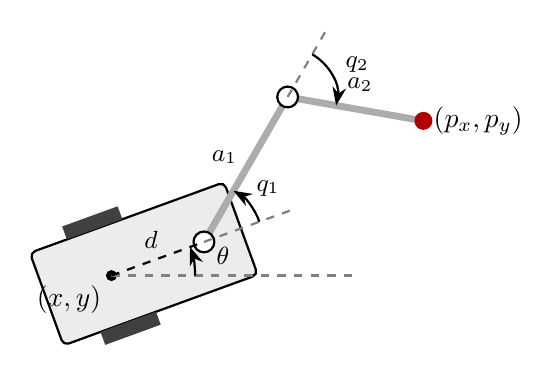
\begin{tikzpicture}[>=Stealth,thick,scale=1.25]
  \coordinate (W) at (0,0);
  \coordinate (M) at (20:1.0);
  \coordinate (P1) at ($(M)+(60:1.7)$);
  \coordinate (P2) at ($(P1)+(-10:1.4)$);
  % base (top view), rotated by theta
  \begin{scope}[rotate=20]
    \draw[rounded corners=2pt,fill=gray!15] (-0.7,-0.5) rectangle (1.4,0.5);
    \fill[black!75] (-0.3,-0.64) rectangle (0.3,-0.5);
    \fill[black!75] (-0.3,0.5) rectangle (0.3,0.64);
  \end{scope}
  \fill (W) circle (1.6pt);
  \node[below left] at (W) {$(x,y)$};
  % reference axis and theta
  \draw[dashed,gray] (W)--(2.5,0);
  \draw[->] (0.85,0) arc[start angle=0,end angle=20,radius=0.85];
  \node at (10:1.15) {\small$\theta$};
  % arm
  \draw[line width=2.5pt,gray!65] (M)--(P1)--(P2);
  \draw[fill=white] (M) circle (3pt);
  \draw[fill=white] (P1) circle (3pt);
  \fill[red!70!black] (P2) circle (2.6pt);
  \node[right] at (P2) {$(p_x,p_y)$};
  % d
  \draw[dashed] (W)--(M);
  \node at ($(W)!0.5!(M)+(110:0.2)$) {\small$d$};
  % q1
  \draw[dashed,gray] (M)--++(20:0.95);
  \draw[->] ($(M)+(20:0.6)$) arc[start angle=20,end angle=60,radius=0.6];
  \node at ($(M)+(40:0.85)$) {\small$q_1$};
  % q2
  \draw[dashed,gray] (P1)--++(60:0.8);
  \draw[->] ($(P1)+(60:0.5)$) arc[start angle=60,end angle=-10,radius=0.5];
  \node at ($(P1)+(25:0.78)$) {\small$q_2$};
  % link names
  \node at ($(M)!0.5!(P1)+(150:0.25)$) {\small$a_1$};
  \node at ($(P1)!0.5!(P2)+(80:0.25)$) {\small$a_2$};
\end{tikzpicture}
\caption{Unicycle base with a planar 2R arm mounted on the sagittal axis at distance $d$ from the wheel center (top view).}
\end{figure}

\paragraph{Direct kinematics for the positioning task.}
\[
\begin{pmatrix}p_x\\ p_y\end{pmatrix}=
\begin{pmatrix}x+d\,c_\theta+a_1c_{\theta q_1}+a_2c_{\theta q_1q_2}\\[2pt]
y+d\,s_\theta+a_1s_{\theta q_1}+a_2s_{\theta q_1q_2}\end{pmatrix},
\]
where $s_{\alpha\dots\gamma}=\sin(\alpha+\dots+\gamma)$ and $c_{\alpha\dots\gamma}=\cos(\alpha+\dots+\gamma)$.

\paragraph{Jacobians.} Differentiating with respect to $\qbase$ and $\qarm$,
\[
\Jbase=\begin{pmatrix}1&0&-d s_\theta-a_1s_{\theta q_1}-a_2s_{\theta q_1q_2}\\
0&1&d c_\theta+a_1c_{\theta q_1}+a_2c_{\theta q_1q_2}\end{pmatrix},\qquad
\Jarm=\begin{pmatrix}-a_1s_{\theta q_1}-a_2s_{\theta q_1q_2}&-a_2s_{\theta q_1q_2}\\
a_1c_{\theta q_1}+a_2c_{\theta q_1q_2}&a_2c_{\theta q_1q_2}\end{pmatrix}.
\]
Multiplying $\Jbase$ by $\Gbase$ (first column: $c_\theta\,\bm e_x+s_\theta\,\bm e_y$; second column: third column of $\Jbase$), the $2\times4$ MM Jacobian is
\[
\Jmm=\begin{pmatrix}
c_\theta & -d s_\theta-a_1s_{\theta q_1}-a_2s_{\theta q_1q_2} & -a_1s_{\theta q_1}-a_2s_{\theta q_1q_2} & -a_2s_{\theta q_1q_2}\\
s_\theta & d c_\theta+a_1c_{\theta q_1}+a_2c_{\theta q_1q_2} & a_1c_{\theta q_1}+a_2c_{\theta q_1q_2} & a_2c_{\theta q_1q_2}
\end{pmatrix}.
\]

\begin{proposition}\label{prop:nosing}
The MM of Example~\ref{ex:uni2r} has no kinematic singularities if $d>0$.
\end{proposition}

\begin{proof}
Call $\bm c_1,\dots,\bm c_4$ the columns of $\Jmm$ and let $\bm u=(c_\theta,s_\theta)$ be the heading direction, $\bm u^\perp=(-s_\theta,c_\theta)$, and $\bm e_k^\perp$ the unit vector perpendicular to the direction of link $k$. Then
\[
\bm c_1=\bm u,\qquad
\bm c_2=d\,\bm u^\perp+a_1\bm e_1^\perp+a_2\bm e_2^\perp,\qquad
\bm c_3=a_1\bm e_1^\perp+a_2\bm e_2^\perp,\qquad
\bm c_4=a_2\bm e_2^\perp .
\]
Therefore $\bm c_3-\bm c_2=-d\,\bm u^\perp$. Since $\bm u$ and $\bm u^\perp$ are orthogonal unit vectors and $d>0$, the vectors $\bm c_1=\bm u$ and $\bm c_3-\bm c_2=-d\,\bm u^\perp$ are linearly independent, so $\mathrm{rank}\,\Jmm=2$ for \emph{every} configuration.
\end{proof}

\paragraph{Comparison with the arm alone.} A direct computation gives
\[
\det\Jarm=a_1a_2\sin q_2 ,
\]
so the 2R arm alone is singular whenever $q_2=0$ (arm fully stretched) or $q_2=\pm\pi$ (arm folded).

\begin{figure}[ht]
\centering
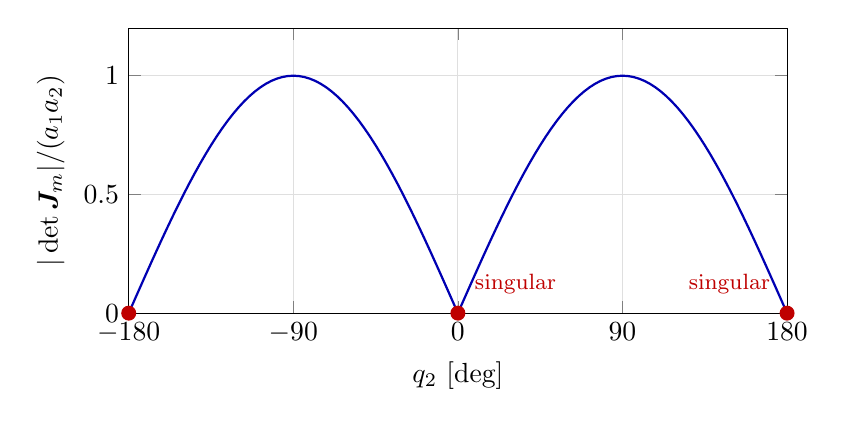
\begin{tikzpicture}
\begin{axis}[width=0.82\textwidth,height=5.2cm,xlabel={$q_2$ [deg]},
  ylabel={$|\det\Jarm|/(a_1a_2)$},xmin=-180,xmax=180,xtick={-180,-90,0,90,180},
  ymin=0,ymax=1.2,domain=-180:180,samples=121,grid=major,grid style={gray!25}]
  \addplot[thick,blue!70!black]{abs(sin(x))};
  \addplot[only marks,mark=*,mark size=2.5pt,red!75!black] coordinates {(-180,0)(0,0)(180,0)};
  \node[red!75!black,font=\footnotesize,anchor=south west] at (axis cs:4,0.04) {singular};
  \node[red!75!black,font=\footnotesize,anchor=south east] at (axis cs:176,0.04) {singular};
\end{axis}
\end{tikzpicture}
\caption{Determinant of the 2R arm Jacobian as a function of $q_2$: the arm alone is singular at $q_2\in\{0,\pm\pi\}$. With the unicycle base ($d>0$) these singularities disappear.}
\end{figure}

\begin{intuition}
At a stretched-out arm configuration the hand cannot move along the arm direction. A mobile base removes this obstruction: driving forward moves the hand along the heading $\bm u$, while \emph{rotating} the base about the wheel center moves the hand along $\bm u^\perp$ with lever arm $d$ (the column $\bm c_3-\bm c_2=-d\bm u^\perp$ in the proof). A unicycle cannot translate sideways, but if the arm is mounted ahead of the wheel axis, a rotation produces a sideways hand velocity anyway. If $d=0$ the lever arm vanishes and this advantage is lost. In words: \emph{adding the degrees of freedom of the base allows removing the singularities of the 2R arm alone.}
\end{intuition}

% =====================================================================
\section{Inverse differential kinematics \emph{(manipulator slides 9--10)}}

\subsection{Redundancy resolution}

Methods for solving inverse differential kinematics in the presence of redundancy (\emph{redundancy resolution}) extend to MMs with minimal adaptation.

\begin{proposition}[Pseudoinverse solution with null-space term]\label{prop:ik}
Let $\Jmm(\bm q)$ have full row rank and let $\dot{\bm y}_d$ be the desired task velocity. Every input $\bm u$ with $\Jmm\bm u=\dot{\bm y}_d$ can be written as
\[
\bm u=\Jmm^\dagger(\bm q)\,\dot{\bm y}_d+\bigl(\bm I-\Jmm^\dagger(\bm q)\Jmm(\bm q)\bigr)\bm u_N ,
\]
for a suitable $\bm u_N$, where $\Jmm^\dagger=\Jmm^T(\Jmm\Jmm^T)^{-1}$ is the pseudoinverse. The first term is the minimum-norm solution; the second term lies in $\ker\Jmm$ and does not affect the task.
\end{proposition}

\begin{proof}
Let $\bm P=\bm I-\Jmm^\dagger\Jmm$. Since $\Jmm\Jmm^\dagger=\bm I$, we get $\Jmm\bm P=\Jmm-\Jmm=\bm O$, so $\Jmm(\Jmm^\dagger\dot{\bm y}_d+\bm P\bm u_N)=\dot{\bm y}_d$ for any $\bm u_N$. Conversely, if $\Jmm\bm u=\dot{\bm y}_d$, take $\bm u_N=\bm u$: then $\Jmm^\dagger\dot{\bm y}_d+\bm P\bm u=\Jmm^\dagger\Jmm\bm u+\bm u-\Jmm^\dagger\Jmm\bm u=\bm u$. Finally $\bm P$ is symmetric and idempotent, i.e.\ the orthogonal projector onto $\ker\Jmm$, and $\Jmm^\dagger\dot{\bm y}_d\in\mathrm{range}(\Jmm^T)\perp\ker\Jmm$, so $\|\bm u\|^2=\|\Jmm^\dagger\dot{\bm y}_d\|^2+\|\bm P\bm u_N\|^2$ is minimised by $\bm P\bm u_N=\bm 0$.
\end{proof}

\begin{intuition}
The set of inputs producing the desired hand velocity is a flat ``affine subspace'': one particular solution plus anything in the kernel. The pseudoinverse picks the smallest one (least effort), and the term $\bm P\bm u_N$ spends the leftover freedom --- the \emph{self-motion} of the robot --- on a secondary goal $H(\bm q)$ (stay away from joint limits, keep the arm well-conditioned, avoid obstacles), without disturbing the hand at all. Think of holding a cup steady while your elbow and torso reposition.
\end{intuition}

\subsection{Why the gradient cannot be used directly}

The null-space term $\bm u_N$ should improve a performance criterion $H(\bm q)$ without affecting the task. For a fixed-base manipulator one would simply take $\bm u_N=\pm\alpha\,\grad H(\bm q)$ (sign $+$ to maximise, $-$ to minimise). For an MM this is not possible: the first $m_b$ components of $\bm u$ are \emph{pseudovelocities}, not generalized velocities, so they cannot be set equal to components of a gradient. Put differently, the nonholonomic constraints on the base prevent motion in the direction of the gradient.

\begin{intuition}
Imagine $H$ increases if the vehicle moves sideways. The gradient points sideways, but a unicycle cannot slide sideways; and even the dimensions do not match ($\grad H$ has $n$ entries, $\bm u$ only $m$). The gradient is a ``wish'' in configuration space; the controls live in a different, smaller space.
\end{intuition}

\subsection{The right choice of \texorpdfstring{$\bm u_N$}{uN}}

To find a suitable $\bm u_N$, look at the time derivative of $H$ along the system motion:
\[
\dot H(\bm q)=\frac{\partial H}{\partial\bm q}\dot{\bm q}=\grad^{\!T}H(\bm q)\,\bm G(\bm q)\,\bm u .
\]
By the Cauchy--Schwarz inequality this is maximised (for given $\|\bm u\|$) when $\bm u$ is aligned with $\bm G^T(\bm q)\grad H(\bm q)$.

\begin{proposition}[Maximum local improvement]\label{prop:uN}
Choosing
\[
\bm u_N=\pm\alpha\,\bm G^T(\bm q)\,\grad H(\bm q)=\pm\alpha\begin{pmatrix}\Gbase^T(\qbase)&\bm O\\ \bm O&\bm I\end{pmatrix}\grad H(\bm q),\qquad\alpha>0,
\]
yields the maximum local improvement of $H(\bm q)$, with corresponding generalized velocity
\[
\dot{\bm q}_N=\bm G(\bm q)\bm u_N=\pm\alpha\,\bm G(\bm q)\bm G^T(\bm q)\grad H(\bm q),
\]
which is the projection of $\pm\alpha\grad H(\bm q)$ onto the subspace of admissible generalized velocities $\mathrm{range}\,\bm G(\bm q)$.
\end{proposition}

\begin{remark}
If the columns of $\bm G$ are orthonormal, $\bm G\bm G^T$ is exactly the orthogonal projector onto $\mathrm{range}\,\bm G$. This is the case for the unicycle, where $\Gbase=\begin{pmatrix}c_\theta&0\\ s_\theta&0\\0&1\end{pmatrix}$ and
\[
\Gbase^T\nabla_{\qbase}H=\begin{pmatrix}c_\theta\,\partial_xH+s_\theta\,\partial_yH\\ \partial_\theta H\end{pmatrix}.
\]
So the forward velocity $v$ follows the component of the gradient along the heading, $\omega$ follows $\partial_\theta H$ (turn to make $H$ grow), and each joint velocity follows $\partial_{q_j}H$. The component of the gradient orthogonal to the heading is simply discarded.
\end{remark}

\begin{remark}[Effect of the projection]
In the resulting control the null-space velocity is actually $\bm P\bm u_N$, not $\bm u_N$. The resulting improvement of $H$ due to this term is $\pm\alpha\,\|\bm P\bm G^T\grad H\|^2$, because $\grad^{\!T}H\,\bm G\bm P\bm G^T\grad H=\|\bm P\bm G^T\grad H\|^2$ ($\bm P$ symmetric idempotent). Hence the projection may reduce the improvement, but never reverses its sign.
\end{remark}

\begin{figure}[ht]
\centering
\begin{tikzpicture}[>=Stealth,thick,scale=1.1]
  \draw[gray!60,dashed] (-1,-0.58)--(5,2.89) node[above right,black]{\small admissible direction (heading)};
  \draw[->,red!70!black,line width=1.3pt] (0,0)--(75:3.1) node[above]{$\pm\alpha\,\nabla H$};
  \draw[->,blue!70!black,line width=1.3pt] (0,0)--(30:2.19) node[below right]{$\dot{\bm q}_N$};
  \draw[dashed,gray] (75:3.1)--(30:2.19);
  \fill (0,0) circle (1.8pt);
  \draw (0.7,0) arc[start angle=0,end angle=30,radius=0.7];
  \node at (0.95,0.17) {\small$\theta$};
\end{tikzpicture}
\caption{Base-only cartoon in the $(x,y)$ plane: the wished motion $\pm\alpha\nabla H$ is projected onto the only direction the unicycle can actually move along (its heading). The orthogonal component is lost.}
\end{figure}

\begin{intuition}
The recipe is ``\emph{do the best you can with the motions you are allowed}''. Compute the gradient as if everything were free, then map it through $\bm G^T$ to obtain the controls that make $\dot H$ as large as possible. Numerical example for the unicycle at $\theta=0$ with $\nabla_{\qbase}H=(2,\,5,\,1)$: the vehicle gets $v=2$ (forward component), $\omega=1$, and the sideways ``$5$'' is ignored. The result is not the ideal improvement ($\|\grad H\|^2$) but the best \emph{admissible} one ($\|\bm G^T\grad H\|^2$).
\end{intuition}

\begin{algorithm}[Redundancy resolution for an MM]\label{alg:ik}
At each control instant:
\begin{enumerate}[leftmargin=*,nosep]
\item compute $\Jmm(\bm q)=(\Jbase\Gbase\ \ \Jarm)$ and its pseudoinverse $\Jmm^\dagger$;
\item compute $\bm u_N=\pm\alpha\,\bm G^T(\bm q)\grad H(\bm q)$;
\item output $\bm u=\Jmm^\dagger\dot{\bm y}_d+(\bm I-\Jmm^\dagger\Jmm)\bm u_N$ and apply $\ubase$ to the base, $\uarm$ to the arm.
\end{enumerate}
\end{algorithm}

% =====================================================================
\section{Kinematic control \emph{(manipulator slide 11)}}

In general, as for manipulators, robust feedback control laws for MMs should be designed on the basis of their \emph{dynamic} model. Kinematic control of MMs gives acceptable performance only if the required velocities are small, so that the inertial couplings between the coordinates of the base and those of the manipulator remain negligible.

A closed-loop inverse kinematic scheme (\emph{kinematic control}) is obtained by adding an error feedback term $\bm K(\bm y_d-\bm y_e)$ to the feedforward term $\dot{\bm y}_d$ in the control of Proposition~\ref{prop:ik}:
\[
\bm u=\Jmm^\dagger(\bm q)\bigl[\dot{\bm y}_d+\bm K(\bm y_d-\ye)\bigr]+\bigl(\bm I-\Jmm^\dagger\Jmm\bigr)\bm u_N ,\qquad \ye=\bm k_e(\bm q).
\]

\begin{proposition}[Task error dynamics]\label{prop:err}
If $\Jmm$ has full row rank along the motion and $\bm K$ is a symmetric positive-definite matrix, the task error $\bm e=\bm y_d-\ye$ obeys $\dot{\bm e}=-\bm K\bm e$ and converges exponentially to zero, irrespective of $\bm u_N$.
\end{proposition}

\begin{proof}
$\dot{\bm e}=\dot{\bm y}_d-\Jmm\bm u=\dot{\bm y}_d-\Jmm\Jmm^\dagger[\dot{\bm y}_d+\bm K\bm e]-\Jmm\bm P\bm u_N=\dot{\bm y}_d-\dot{\bm y}_d-\bm K\bm e=-\bm K\bm e$, using $\Jmm\Jmm^\dagger=\bm I$ and $\Jmm\bm P=\bm O$.
\end{proof}

\begin{figure}[ht]
\centering
\resizebox{\textwidth}{!}{%
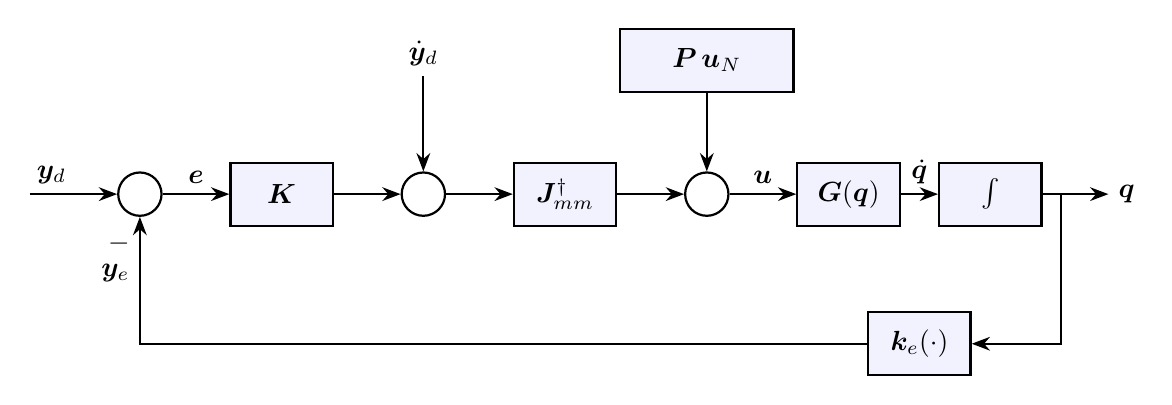
\begin{tikzpicture}[>=Stealth,thick,
  blk/.style={draw,rectangle,minimum width=1.3cm,minimum height=0.8cm,fill=blue!5},
  sm/.style={draw,circle,inner sep=1pt,minimum size=0.55cm}]
  \node[sm] (s1) at (0,0) {};
  \node[blk] (K) at (1.8,0) {$\bm K$};
  \node[sm] (s2) at (3.6,0) {};
  \node[blk] (Jd) at (5.4,0) {$\Jmm^\dagger$};
  \node[sm] (s3) at (7.2,0) {};
  \node[blk] (G) at (9.0,0) {$\bm G(\bm q)$};
  \node[blk] (I) at (10.8,0) {$\int$};
  \node[blk] (ke) at (9.9,-1.9) {$\bm k_e(\cdot)$};
  \node[blk,minimum width=2.2cm] (uN) at (7.2,1.7) {$\bm P\,\bm u_N$};
  \draw[->] (-1.4,0)--(s1) node[pos=0.25,above]{$\bm y_d$};
  \draw[->] (s1)--(K) node[midway,above]{$\bm e$};
  \draw[->] (K)--(s2);
  \draw[->] (3.6,1.5) node[above]{$\dot{\bm y}_d$}--(s2);
  \draw[->] (s2)--(Jd);
  \draw[->] (Jd)--(s3);
  \draw[->] (uN)--(s3);
  \draw[->] (s3)--(G) node[midway,above]{$\bm u$};
  \draw[->] (G)--(I) node[midway,above]{$\dot{\bm q}$};
  \draw[->] (I)--(12.3,0) node[right]{$\bm q$};
  \draw[->] (11.7,0)|-(ke);
  \draw[->] (ke)-|(s1) node[pos=0.78,left]{$\ye$} node[pos=0.97,below left]{$-$};
\end{tikzpicture}}
\caption{Kinematic control scheme of an MM: error feedback plus feedforward through $\Jmm^\dagger$, with a null-space term for the secondary criterion.}
\end{figure}

\begin{intuition}
It is a ``proportional controller in task space'': the error between desired and actual hand pose is turned into a corrected desired hand velocity, which the pseudoinverse then distributes among base and arm. Because everything is expressed through $\Jmm^\dagger$, the same law drives the base wheels and the arm joints in a coordinated way; the null-space part moves the robot ``behind the scenes''. The assumption of small velocities is the price of ignoring dynamics: if the base accelerates hard, its inertia reacts on the arm and the kinematic prediction is no longer accurate.
\end{intuition}

\begin{remark}
Near singularities $\Jmm^\dagger$ becomes very large. A common practical remedy (not covered here) is the damped pseudoinverse $\Jmm^T(\Jmm\Jmm^T+\lambda^2\bm I)^{-1}$. By Proposition~\ref{prop:nosing}, for the unicycle with a 2R arm and $d>0$ this issue does not arise for the positioning task.
\end{remark}

% =====================================================================
\section{Summary}

\subsection*{Regulation}

\begin{table}[ht]
\centering
\renewcommand{\arraystretch}{1.35}
\begin{tabular}{@{}>{\raggedright\arraybackslash}p{2.6cm}>{\raggedright\arraybackslash}p{6.0cm}>{\raggedright\arraybackslash}p{6.2cm}@{}}
\toprule
 & \textbf{Cartesian regulation} & \textbf{Posture regulation}\\
\midrule
Goal & reach $(0,0)$, any orientation & reach $(0,0,0)$\\
Coordinates & $\bm e_p$, projection on $\bm n$, pointing error $\gamma$ & polar: $\rho,\gamma,\delta=\gamma+\theta$\\
Design approach & geometric projection on sagittal axis & constructive Lyapunov design (cross-term cancellation)\\
Control law & $v=k_1\rho\cos\gamma$, $\omega=k_2\gamma$ & $v=k_1\rho\cos\gamma$, $\omega=k_2\gamma+k_1\frac{\sin\gamma\cos\gamma}{\gamma}(\gamma+\delta)$\\
Lyapunov function & $V=\frac12(x^2+y^2)$ (PSD in $\R^3$, zero on $\theta$-axis) & $V=\frac12(\rho^2+\gamma^2+\delta^2)$ (PD in polar coordinates)\\
$\dot V$ & $-k_1(x\cos\theta+y\sin\theta)^2\le0$ & $-k_1\cos^2\!\gamma\,\rho^2-k_2\gamma^2\le0$\\
Invariance tool & Barbalat (LaSalle fails: sublevel sets non-compact) & Barbalat (+ closed-loop analysis for $\delta$)\\
Steady state & broadside scenario ($\gamma=\pm\pi/2\implies\omega\ne0$) ruled out & full state convergence $\rho,\gamma,\delta\to0$\\
Final heading & uncontrolled & $\theta\to0$\\
Maneuvers & at most one backup & at most one backup\\
Continuity & discontinuous (Atan2 jump) & discontinuous at origin (Brockett); never met in practice\\
\bottomrule
\end{tabular}
\caption{Cartesian versus posture regulation of the unicycle.}
\end{table}

\subsection*{Mobile manipulators}

\begin{table}[ht]
\centering
\renewcommand{\arraystretch}{1.3}
\begin{tabular}{@{}>{\raggedright\arraybackslash}p{3.2cm}>{\raggedright\arraybackslash}p{6.4cm}>{\raggedright\arraybackslash}p{5.2cm}@{}}
\toprule
\textbf{Topic} & \textbf{Result} & \textbf{Key point}\\
\midrule
Configuration & $\bm q=(\qbase,\qarm)$, $n=n_b+n_m$ & wheeled base + articulated arm\\
Kinematic model & $\dot{\bm q}=\mathrm{diag}(\Gbase,\bm I)\,\bm u$, $\bm u=(\ubase,\uarm)$ & driftless; base has $m_b<n_b$ pseudovelocities\\
Controllability & iff the base is controllable & arm joints add free directions\\
Differential kinematics & $\dot{\bm y}_e=(\Jbase\Gbase\ \ \Jarm)\,\bm u=\Jmm\bm u$ & some entries are not partial derivatives\\
Redundancy & typically $m_b+n_m>6$ & secondary criterion $H(\bm q)$\\
Singularities (unicycle+2R) & none if $d>0$ & arm alone singular at $\sin q_2=0$\\
Inverse diff.\ kinematics & $\bm u=\Jmm^\dagger\dot{\bm y}_d+(\bm I-\Jmm^\dagger\Jmm)\bm u_N$ & min.\ norm + null-space term\\
Null-space term & $\bm u_N=\pm\alpha\,\bm G^T\grad H$ & \emph{not} $\pm\alpha\grad H$ (pseudovelocities)\\
Kinematic control & $\bm u=\Jmm^\dagger[\dot{\bm y}_d+\bm K(\bm y_d-\ye)]+\dots$ & $\dot{\bm e}=-\bm K\bm e$; low speeds only\\
\bottomrule
\end{tabular}
\caption{Summary of the main results on mobile manipulators.}
\end{table}

\begin{table}[ht]
\centering
\renewcommand{\arraystretch}{1.3}
\begin{tabular}{@{}lcc@{}}
\toprule
 & \textbf{Fixed-base manipulator} & \textbf{Mobile manipulator}\\
\midrule
Inputs & $\dot{\bm q}_m$ & $(\ubase,\uarm)$, pseudovelocities for the base\\
Task Jacobian & $\Jarm$ & $\Jmm=(\Jbase\Gbase\ \ \Jarm)$\\
Null-space term & $\pm\alpha\grad H$ & $\pm\alpha\,\bm G^T\grad H$\\
Workspace & limited by the arm & extended by base motion\\
Singularities & arm singularities & removable (e.g.\ $d>0$)\\
\bottomrule
\end{tabular}
\caption{Fixed-base versus mobile manipulators.}
\end{table}

\subsection*{Key take-aways}
\begin{enumerate}[leftmargin=*]
\item Nonholonomic WMRs admit no universal controllers: tracking schemes need persistent trajectories ($v_d(t)\ge v_{\min}>0$), and tracking a trajectory that stops in $\bm q_d$ fails (linearization is uncontrollable at rest, and error-dynamics laws tend to infinity), so regulation needs dedicated laws.
\item Cartesian regulation uses $v=k_1\bm e_p^T\bm n$ and $\omega=k_2\gamma$; $V$ is only semidefinite in $\R^3$ (unbounded sublevel sets along $\theta$ prevent LaSalle), so Barbalat's lemma proves $\bm e_p^T\bm n\to0$; analyzing steady state rules out broadside alignment ($\omega\ne0$) and proves $(x,y)\to0$, while the final orientation is not controlled.
\item Posture regulation uses polar coordinates and a constructive Lyapunov synthesis canceling the cross-coupling term in $\dot V$; Barbalat's lemma proves full convergence $x,y,\theta\to0$. By Brockett's theorem any time-invariant posture stabilizer must be discontinuous, though the origin singularity is never met in practice.
\item A mobile manipulator has a block-diagonal kinematic model, is controllable iff its base is, and has $\Jmm=(\Jbase\Gbase\ \ \Jarm)$; the base DOFs can remove arm singularities (unicycle + 2R with $d>0$).
\item Redundancy is resolved with $\bm u=\Jmm^\dagger\dot{\bm y}_d+(\bm I-\Jmm^\dagger\Jmm)\bm u_N$ with $\bm u_N=\pm\alpha\,\bm G^T\grad H$ (not the raw gradient), and kinematic control with $\bm K(\bm y_d-\ye)$ gives $\dot{\bm e}=-\bm K\bm e$ at low speeds.
\end{enumerate}

\end{document}